\documentclass{ucbthesis}

\usepackage{amsfonts}
\usepackage{amssymb}
\usepackage{biblatex}
\usepackage{color}
\usepackage{graphicx}
\usepackage{hyperref}
\usepackage{listings}
\usepackage{multirow}
\usepackage{subcaption}
\usepackage{times}
\usepackage[T1]{fontenc}

\lstset{
  showspaces=false,
  showtabs=false,
  breaklines=true,
  showstringspaces=false,
  breakatwhitespace=true,
  escapeinside={(*@}{@*)},
  basicstyle=\scriptsize\ttfamily,
  columns=fullflexible,
  morekeywords={maybe_downsample, maybe_skip}
}

%% \def\dsp{\def\baselinestretch{2.0}\large\normalsize}
%% \dsp

\bibliography{thesis}

\begin{document}

\title{ A Proposal for Adaptive Wide-area Streaming Analytics }

\author{ Ben Zhang }
\degreesemester{XX}
\degreeyear{XXXX}
\degree{Doctor of Philosophy}
\chair{Professor John Wawrzynek}
\othermembers{Professor Edward A. Lee \\
  Professor Sylvia Ratnasamy \\
  Professor John Chuang}
\field{Computer Science}
\campus{Berkeley}
\numberofmembers{3}

\maketitle
%% \approvalpage
%% \copyrightpage

\newcommand{\sysname}{AdaptiveStream}

\definecolor{todo}{rgb}{1, 0, 0}
\definecolor{ben}{rgb}{0.5, 0.5, 0.0}
\definecolor{xin}{rgb}{0.0, 0.5, 0.5}

\newtoggle{anonymous}
\toggletrue{anonymous}
%\togglefalse{anonymous}

\newtoggle{comments}
\toggletrue{comments}
% \togglefalse{comments}

\iftoggle{comments} {
  % show comments with the corresponding color
  \newcommand {\ben}[1]{{\color{ben}\bf{BZ: #1}\normalfont}}

  \newcommand {\todo}[1]{{\color{todo}TODO: #1}\normalfont}
}{
  % do not show comments
  \newcommand {\ben}[1]{}

  \newcommand {\todo}[1]{}
}

\newcommand{\squishlist}{
  \begin{list}{$\bullet$}
    { \setlength{\itemsep}{0pt}
      \setlength{\parsep}{3pt}
      \setlength{\topsep}{3pt}
      \setlength{\partopsep}{0pt}
      \setlength{\leftmargin}{1.5em}
      \setlength{\labelwidth}{1em}
      \setlength{\labelsep}{0.5em} } }
  \newcommand{\squishend}{
  \end{list}  }

\newcommand{\boldhead}[1]{\vspace{0.5em}\noindent\textbf{#1}}

\newcommand{\para}[1]{\vspace{0.6em}\noindent\textbf{#1}}
\newcommand{\paraf}[1]{\vspace{0.1em}\noindent\textbf{#1}}

\newcommand{\specialcell}[2][c]{%
  \begin{tabular}[#1]{@{}c@{}}#2\end{tabular}}

\renewcommand*\chapterautorefname{Chapter}
\renewcommand*\sectionautorefname{Section}
\renewcommand*\subsectionautorefname{Section}
\renewcommand*{\equationautorefname}{Eq.}
\renewcommand*{\figureautorefname}{Fig.}

%%% Local Variables:
%%% mode: latex
%%% TeX-master: "sigcomm2017"
%%% End:

%%% Local Variables:
%%% mode: latex
%%% TeX-master: "thesis"
%%% End:


\begin{abstract}

  The swarm refers to the vast collection of networked sensors and actuators
  installed in our connected world. Many swarm applications generate, transport,
  distill, and process large streams of data across the wide area in real
  time. The increasing volume of data generated at the edge challenges the
  existing approaches of directly connecting devices to the cloud.

  This thesis begins with an overview of emerging swarm and the architecture
  design trends for swarm applications. The swarm faces challenges from the
  scarce and variable WAN bandwidth and the heterogeneous compute environment
  (from low-power microcontrollers to powerful compute units). When network
  resources or compute resources are insufficient, non-adaptive applications
  will suffer from increased latency or degraded accuracy. Existing approaches
  that support adaptation either require extensive developer effort to write
  manual policies or are limited to application-specific solutions.

  This thesis proposes a systematic and quantitative approach to build adaptive
  swarm applications. The solution has three stages: (1) a set of programming
  abstractions that allow developers to express adaptation options; (2) an
  automatic profiling tool that learns an accurate profile to characterize
  resource demands and application performance; (3) a runtime system responsive
  to environment changes, maximizing application performance guided by the
  learned profile.

  We evaluate our methodology with adaptations to network resources and compute
  resources. For network resources, we present a complete design and
  implementation of the framework \awstream{} and several swarm applications:
  pedestrian detection, augmented reality, and monitoring log analysis. Our
  experiments show that all applications can achieve sub-second latency with
  nominal accuracy drops. For compute resources, we focus on improving the
  profiling efficiency---using Bayesian Optimization to address the large
  parameter space and profile transfer to address device heterogeneity.

\end{abstract}

%%% Local Variables:
%%% mode: latex
%%% TeX-master: "thesis"
%%% End:


\pagestyle{headings}
\chapter{Introduction}

Wide-area streaming analytics are becoming pervasive, especially with the
emerging Internet-of-Thing (IoT) applications. Large cities such as New York,
Beijing and Seattle are deploying millions of cameras for traffic
control~\cite{london.surveillance,skynet}. Retails stores and critical areas
such as railway stations are also being monitored for abnormal
activities. Buildings are increasingly instrumented with a wide variety of
sensors to improve building energy use, occupant comfort, reliability and
maintenance~\cite{krioukov2012building}. Geo-distributed infrastructure, such as
Content Delivery Network (CDN), needs to analyze user requests (machine logs)
and optimize data placement to improve delivery efficiency. In these problems,
the data collected at the edge needs to be transported acoross the wide-area and
analyzed in real-time.

Existing stream processing for ``big data,'' such as
Borealis~\cite{abadi2005design}, Storm~\cite{toshniwal2014storm}, or Spark
Streaming~\cite{zaharia2012discretized}, only work in the context of a single
cluster, where the bandwidth is sufficient (or at least easy to
provision). While they are the perfect back end for analyzing streams once data
arrive, in the wide-area, the network, with scarce and variable bandwidth,
easily becomes the bottleneck \cite{rabkin2014aggregation}. What's worse, the
growth rate of wide-area network capacity is not keeping up with the increasing
rate of traffic~\cite{index2013zettabyte}.

When facing situations where the bandwidth is not sufficient, applications
deployed today either choose a conservative setting (e.g.\,only delivering 360p
videos) or leave their fate to the underlying transport layer: (1) in the case
of TCP, the sender will be blocked and data are backlogged, leading to severe
delay; (2) in the case of UDP, uncontrolled packet loss occurs, leading to
application performance drop. Instead of ``suffering'' from a degraded network,
applications can act proactively by adjusting their behavior: reducing the data
rate to ensure that important data are delivered in time.

The idea of adapting data rate for data freshness is not new. Multimedia
applications and their adaptations~\cite{michalos2012dynamic,
  schulzrinne1998real} have been extensively studied in the past because their
high demands on the network are rarely met. However, because of the goal to
improve \textbf{user experience}, their adaptation strategies are not
necessarily optimal for streaming analytics. For example, humans can tolerate
losses on video frame details but expect a smooth frame transition---at least 25
frames per second (FPS). But many vision analytics are based on algorithms that
extract edge information from a frame---they will perform poorly after an
aggressive quantization.

The observation that different applications demand different strategies in order
to achieve the optimal adaptation calls for a system-level approach. In this
proposal, I present the design and implementation of \sysname{}, an adaptive
stream processing system for the wide-area. Under normal operations, \sysname{}
applications work with maximal data fidelity; when the network's capacity
changes, applications will react by controlling the level of degradation:
trading data fidelity for freshness.

Although the basic idea behind degradation is intuitive, realizing them in
practice is non-trivial. Firstly, as has been discussed earlier, different
degradations have different impacts across applications and data
distributions. Secondly, each degradation is often more than a binary decision;
they are often parameterized with a wide range of tuning space. It's not always
possible to derive a close-form analytical relationship between the degradation
parameter and its impact on the bandwidth and accuracy. What's more, real-world
applications often have multiple dimensions to tune---prohibiting a manual
exploration of all the design space. Take video analytics as an example,
reducing image resolution, frame rate or changing the video encoding quality are
all possible degradation operations that affect data rate and application
accuracy; and even the impact of each individual operation is not immediately
obvious for developers. These challenges are elaborated
in~\autoref{sec:challenges}.

To address these challenges, \sysname{} employs a data-driven empirical-analysis
approach that's analogous to machine learning.  First, \sysname{} separates
application logic from adaptation strategies by providing a clean abstraction
(\texttt{maybe} APIs) for developers: this allows expressibility without
burdening the developers for an exact strategy. \sysname{} then profiles the
application using representative datasets and application-specific utility
functions to ``learn'' the optimal strategies under different network
conditions. The profile is then used to guide the runtime adaptation, for which
\sysname{} provides all the necessary ``plumbing'' modules to without
application developers' effort. In \autoref{sec:architecture}, I will present a
detailed description of \sysname{}'s architecture.

To study and validate the effect of degradation, I've a prototype framework and
three real-world applications using \sysname{}: a street surveillance
application performing pedestrian detection, an augmented reality application
recognizing everyday objects and a distributed top-k application analyzing web
server access logs. The first two video streaming applications have three
degradation operations: resolution, frame rate and video encoding quality. For
the distributed top-k application, two degradation operations are envolved: N in
a local top-N operation and T as a local threshold. \autoref{sec:build-appl}
discusses the considerations and details about the prototype.

The evaluation shows that the offline profiling is able to explore the design
space for all three applications and generates the adaptation Pareto-optimal
strategies that was not achievable with developer configurations or only a
single degradation operation. These profiles offer a quantitative understanding
of each application's behavior. During runtime, \sysname{} applications are
compared against traditional transport protocols including TCP and UDP with a
controlled experiment. When the network capacity drops, TCP creates a severe
delay; and the delay increases linearly as time goes; for UDP, a severe packet
loss makes the application unusable. Applications built with \sysname{} handles
the network variation gracefully: video streaming analytics is able to keep the
latency bounded with 2 seconds and the accuracy higher than 80\%. For the top-k
application, although the feedback is less frequent and adaptation is not always
immediate, the worst-case latency is 12 seconds at most and the accuracy is
mostly above 75\%.

To this end, this thesis makes the following contributions:

\squishlist    %% \begin{itemize}
\item An in-depth study of wide-area streaming applications in the case of
  network resource variation.
\item The proposal of novel APIs to allow for a design space exploration between
  bandwidth and accuracy with minimal developer effort.
\item A prototype implementation that demonstrates application profiling and
  runtime adaptation.
\item Thorough evaluations based on three real-world applications under
  different scenarios.
\squishend %% \end{itemize}

\section{Motivating Applications}
\label{sec:motiv-appl}

While there is a variety of wide-area streaing applications, we discuss three
applications with their implications.

\para{Video Surveillance:} We envisage a city-wide monitoring system that
aggregates camera feeds (both stationary ground cameras and moving aerial
vehicles) and analyzes video streams in real-time for surveillance, anomaly
detection or business intelligence~\cite{oh2011large}. While traditionally human
labors are involved in analyzing abnormal activities, recent advances in
computer vision and deep learning has dramatically increased the accuracy for
automatic analysis of visual scenes, such as pedestrian
detection~\cite{dollar2012pedestrian}, vehicle tracking~\cite{coifman1998real},
or facial recognition to locate people of
interest~\cite{Lu:2015:SHF:2888116.2888245, parkhi2015deep}.
% \cite{gantz2012digital}

\para{Electrical Grid Monitoring:} While traditional environmental sensors are
slow~\cite{atzori2010internet}, we are seeing an increasing trend with
high-frequency, high-precision sensors being deployed. For example, the
microsynchophasors monitoring system for the electrical grid consists of a
network of 1000 devices; each produces 12 streams of 120 Hz high-precision
values accurate to 100 ns. This amounts to 1.4 million points per second that
requires specialized timeseries database~\cite{andersen2016btrdb}.

\para{Log Analysis:} Large organizations today are managing 10--100s of
datacenters (DCs) and edge clusters worldwide~\cite{calder2013mapping}. While
most log analysis today runs in a batch mode and at most on a daily basis, there
is a trend in analyzing logs in real time for quicker
optimization~\cite{alspaugh2014analyzing}. For example, by analyzing the access
logs in real time, a content distribution network (CDN) can improve the overall
delivery efficiency with optimized data placement.

\vspace{0.5em}

These applications share a similar structure: a large volume of data generated
at the edge need to be transported across the wide area network for real time
analysis. Because of the limited network resources in the wide area, they will
face practical issues when deployed at a scale.

\section{Wide-Area Bandwidth Characteristics}
\label{sec:making-case-adapt}

\begin{figure}
  \centering
  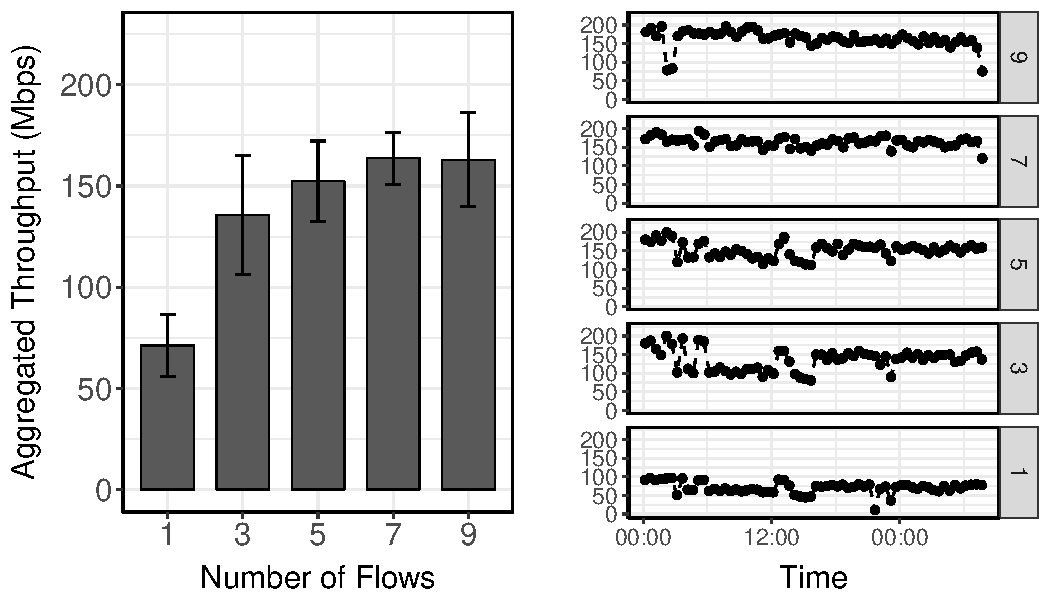
\includegraphics[width=.95\linewidth]{figures/europe-to-us-west.pdf}
  \caption{Bandwidth measurement between Amazon EC2 sites (from Ireland to
    California). Note the time-series plot has a resolution of 30 minutes; each
    point is more than a short period of transient degradation.}
  \label{fig:bw}
\end{figure}

To understand the bandwidth characteristics in the wide-area, I conducted a
simple measurement using Amazon EC2. iPerf~\cite{iperf} was used to measure the
pair-wise bandwidth between four geo-distributed sites throughout the day. The
measurement shows large variance in the measured bandwidth and one such pair of
sites is shown in \autoref{fig:bw}. Regardless of the number of
flows\footnote{EC2 has a per-flow and per-VM rate
  limiting~\cite{zhang2016guaranteeing}.}, there exist occasions when the
available bandwidth is almost halved. Generally speaking, the back-haul links
between EC2 sites are better (if not at least representative) in comparison to
the overall wide-area link quality. This varying nature poses real challenges to
the realization and successful deployment of wide-area streaming applications.

\section{Making the Case for a System Approach}
\label{sec:bat}

When facing insufficient network bandwidth, applications that do not adapt will
suffer severe performance penalty: such as a backlog of data for TCP or
uncontrolled packet loss for UDP. Instead of giving up control to the underlying
transport layer, applications can react and adapt their behaivors to the
resource changes.

While adaptive streaming exists in certain application domains, there has not
been a general solution. Consider video streaming applications that have been
extensively studied in the literature. There are a plethora of encoding
techniques~\cite{richardson2011h, grange2016vp9} with adaptive
strategies~\cite{yin2015control, michalos2012dynamic, pantos2016http}, however,
their primary goal is to optimize end-user quality of experience (QoE).  When
end users consume a video clip, a smooth video is often more enjoyable than
videos with intermittent pauses, even though each pause has crisp images.

Optimizing for a single goal doesn't work for our target applications. Each
video streaming application have its own goal, entailing different adaptive
strategies for different applications. For example, some computer vision
detection algorithms rely on the edge information~\cite{canny1986computational,
  lowe2004distinctive, viola2001rapid} while object tracking applications works
best when the inter-frame difference is small~\cite{allen2004object}.

\begin{figure}
  \centering
  \includegraphics[width=\linewidth]{figures/image-example.pdf}
  \caption{The frame difference between two images with one second difference.
    These are two different deployment scenarios: a stationary camera in a far
    field (upper) and a mobile camera for nearby objects (lower).}
  \label{fig:image-eg}
\end{figure}

Furthermore, even similar applications, when used in different context, requires
different strategy. \autoref{fig:image-eg} offers an example. A pedestrian
detection application is deployed on a ground stationary camera in a far-field
view. When taking pedestrian walking speed into consideration, there is so
little difference between frames that it's not necessary to guarantee a high
frame rate. But because the camera is far from the targets, it's crucial to have
a high-resolution and sharp image. On the other hand, object recognition on a
mobile phone captures nearby objects. Due to the movement of the camera,
reducing frame rate will introduce significant errors. \autoref{fig:motiv} shows
the different rate in accuracy drop when image resolution or frame rate is
reduced for the two use cases.

\begin{figure}
  \centering
  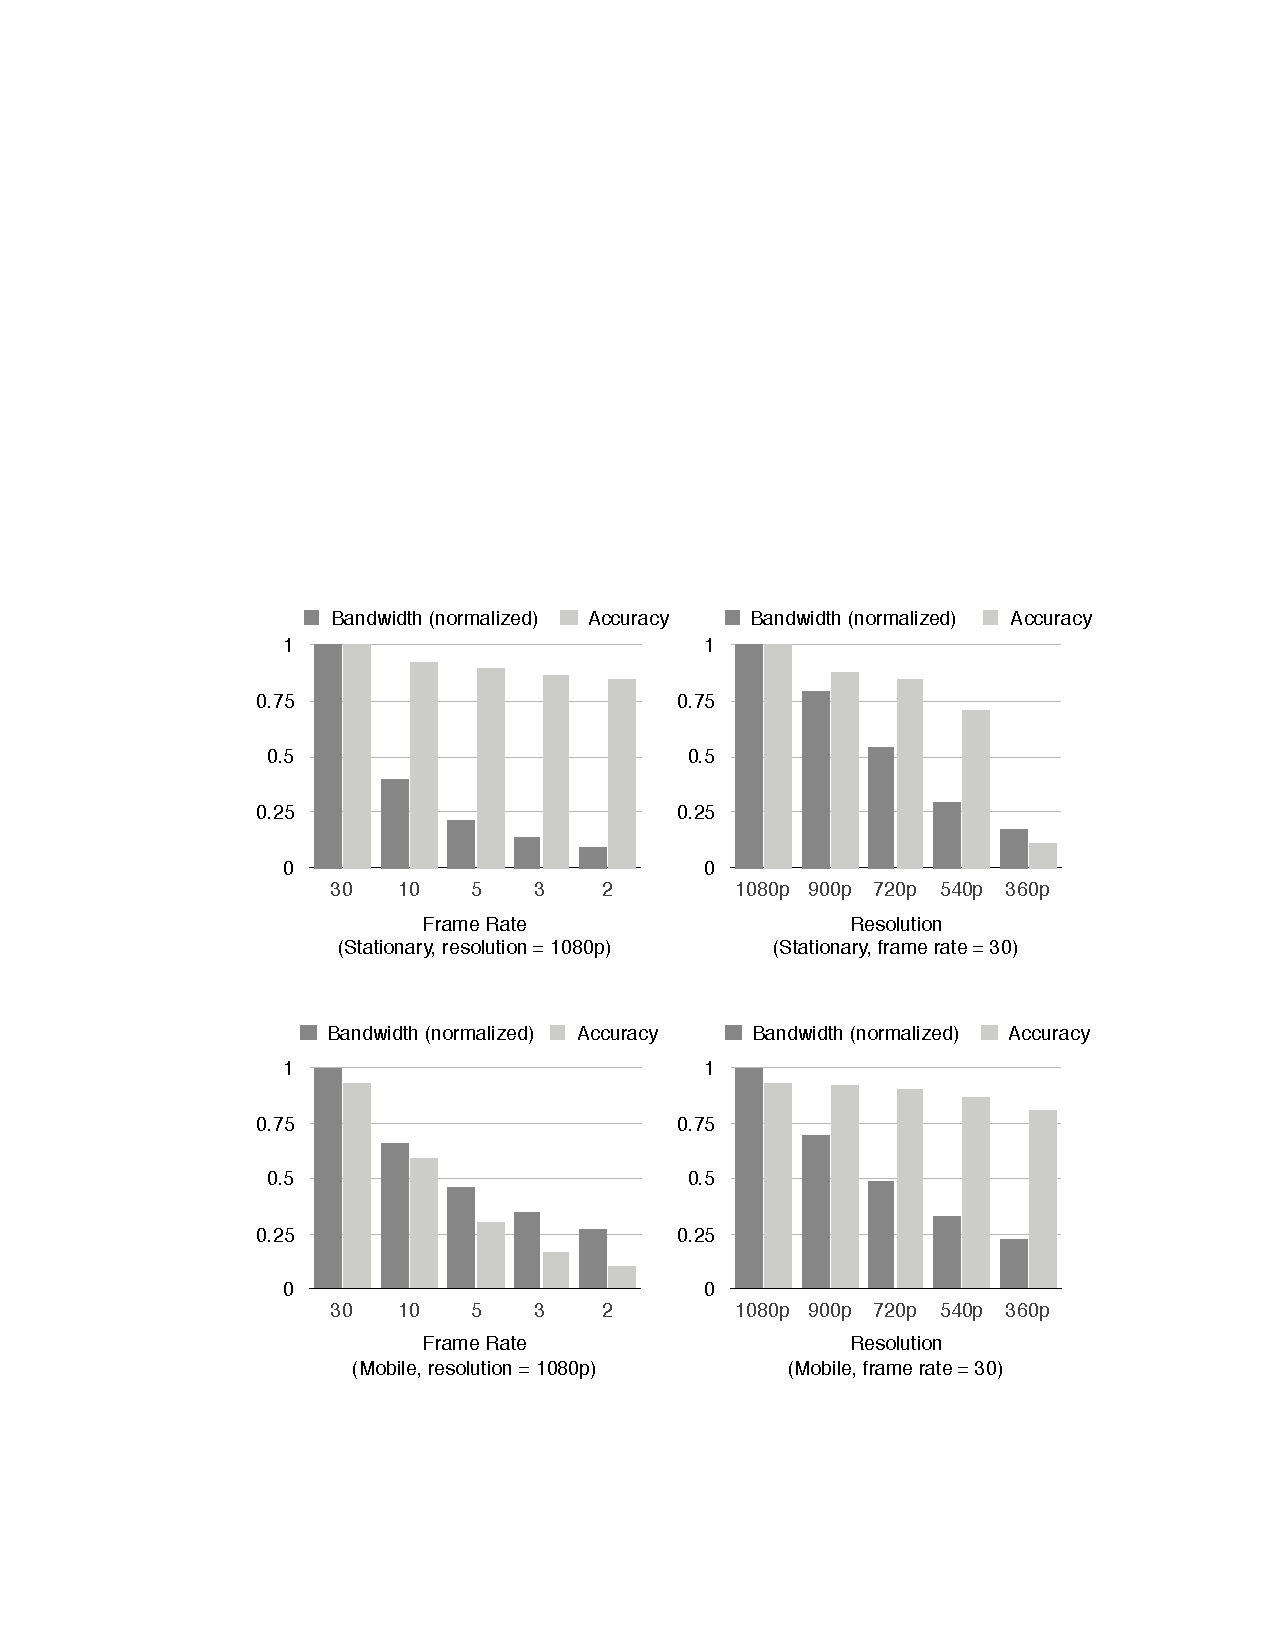
\includegraphics[width=\linewidth]{figures/motiv.pdf}
  \caption{Horizontally, how reducing the frame rate or resolution affects the
    bandwidth requirement and appliation accuracy. Vertically, how the same
    degradation have different impact for different data characteristics; the
    upper figures are for a stationary camera deployment while the lower figures
    are for mobile applications.}
  \label{fig:motiv}
\end{figure}

This motivates us to take a system-level approach that synthesize different
adaptation strategies for different queries and contexts.

\section{Related Work}
\label{sec:related-work}

\paraf{Stream processing systems:} Streaming databases, such as
Borealis~\cite{abadi2005design},
TelegraphCQ~\cite{chandrasekaran2003telegraphcq}, are the early academic
explorations. They pioneered the usage of dataflow models with specialized
operators for stream processing. Recent research projects and open-source
systems, such as MillWheel~\cite{akidau2013millwheel},
Storm~\cite{toshniwal2014storm}, Heron~\cite{kulkarni2015twitter}, Spark
Streaming~\cite{zaharia2012discretized}, Apache Flink~\cite{carbone2015apache},
primary focus on fault-tolerant streaming in the context of a single
cluster. While this thesis has a large debt to the prior streaming work,
\sysname{} is designed for the wide-area and explicitly trades data fidelity for
data freshness; many other stream processing systems choose to throttle the
source when backpressure happens~\cite{kulkarni2015twitter}.

\para{WAN-aware:} There is a growing interest in building systems that optimizes
data transfers for the wide area, such as GDA~\cite{pu2015low},
Clarinet~\cite{viswanathan2016clarinet} and OWAN~\cite{jin2016optimizing}.  Most
of these works focus on one-time queries or operations (such as data
transfer). JetStream~\cite{rabkin2014aggregation} is the first that studies
streaming analytics in wide area and proposes to use structured storage (data
cubes) and explicit degradation policies. While JetStream has demonstrated
application responsiveness with hand-written degradation policy, these policies
are often developer heuristics that are not backed up by measurements. This
thesis extends the idea of degradation with an automatic policy synthesis.

\para{Approximate analytics:} The idea of degrading computation fidelity for
responsiveness has also ben explored in other context, primarily SQL
queries. Online aggregation~\cite{hellerstein1997online},
BlinkDB~\cite{agarwal2013blinkdb} and GRASS~\cite{ananthanarayanan2014grass}
speed up queries with partial data based on statistical models of SQL
operators. \sysname{} supports arbitrary data processing pipelines where no
close-form solution exists to evalute the impact of a particular degradation.

\para{Adaptive video streaming:} This is both an active research
topic~\cite{sun2016cs2p, yin2015control} with many trending industrial efforts.
Because they target at video delivery for web applications, many have chosen to
tune HTTP protocols for video adaptation, such as HLS~\cite{pantos2016http} by
Apple and DASH~\cite{michalos2012dynamic} as the new standard. The main
technique is to adjust the video resolution and encoding bitrate but they often
guarantee a smooth video with high frame rate (at least 25 FPS). This thesis
generalize the adaptation to the wider range of streaming analytics and allow
more custom control over what parameter to be adjusted. \sysname{} applications
can be built upon existing techniques (such as H.264~\cite{richardson2011h} and
VP9~\cite{grange2016vp9}) instead of reinventing the wheel.

%%% Local Variables:
%%% mode: latex
%%% TeX-master: "thesis"
%%% End:

\chapter{\sysname{} Design}
\label{sec:system-design}

In this chapter, I present the design of \sysname{}. The primary goal of
\sysname{} is to enable applications with the ability to adapt its communication
while maximizing its utility.

\section{Challenges}
\label{sec:challenges}

\noindent There are four challenges in realizing \sysname{}.

\para{C1: Diverse application and data:} As discussed in~\autoref{sec:bat}, the
best adaptation scheme is often application- and context-specific
optimizations. It becomes important to separate individual application logic
from specific degradation strategy as well as the concrete mechanisms.

\para{C2: No analytical solutions:} Unlike SQL queries whose demand and accuracy
can typically be estimated using analytical models~\cite{cormode2012synopses},
many of our streaming applications are dealing with unstructure data using
either use blackbox operations (such as H.264 encoding) or non-linear operators
(such as thresholding). The effect of these degradations is not immediately
available.

\para{C3: Multi-dimensional exploration:} Real-world applications typically have
more than one tunable parameters; leading to a combinatorial space for
exploration. In addition, these parameters are not necessarily orthognal.  The
optimal degradation strategies may only be achievable when more than one
degradation is in effect.

\para{C4: Runtime adaptation at application layer:} Although recent work on
resource reservation makes it possible to guarantee quality of service with new
IP or MAC layer protocols in LAN (e.g. TSN~\cite{johas2013heterogeneous}), we
target at WAN analytics where most of the infrastructure is owned by others and
shared among many users. An application-layer solution is in favor to those that
require special hardware or software upgrade.

\section{System Architecture}
\label{sec:architecture}

\begin{figure*}
  \centering
  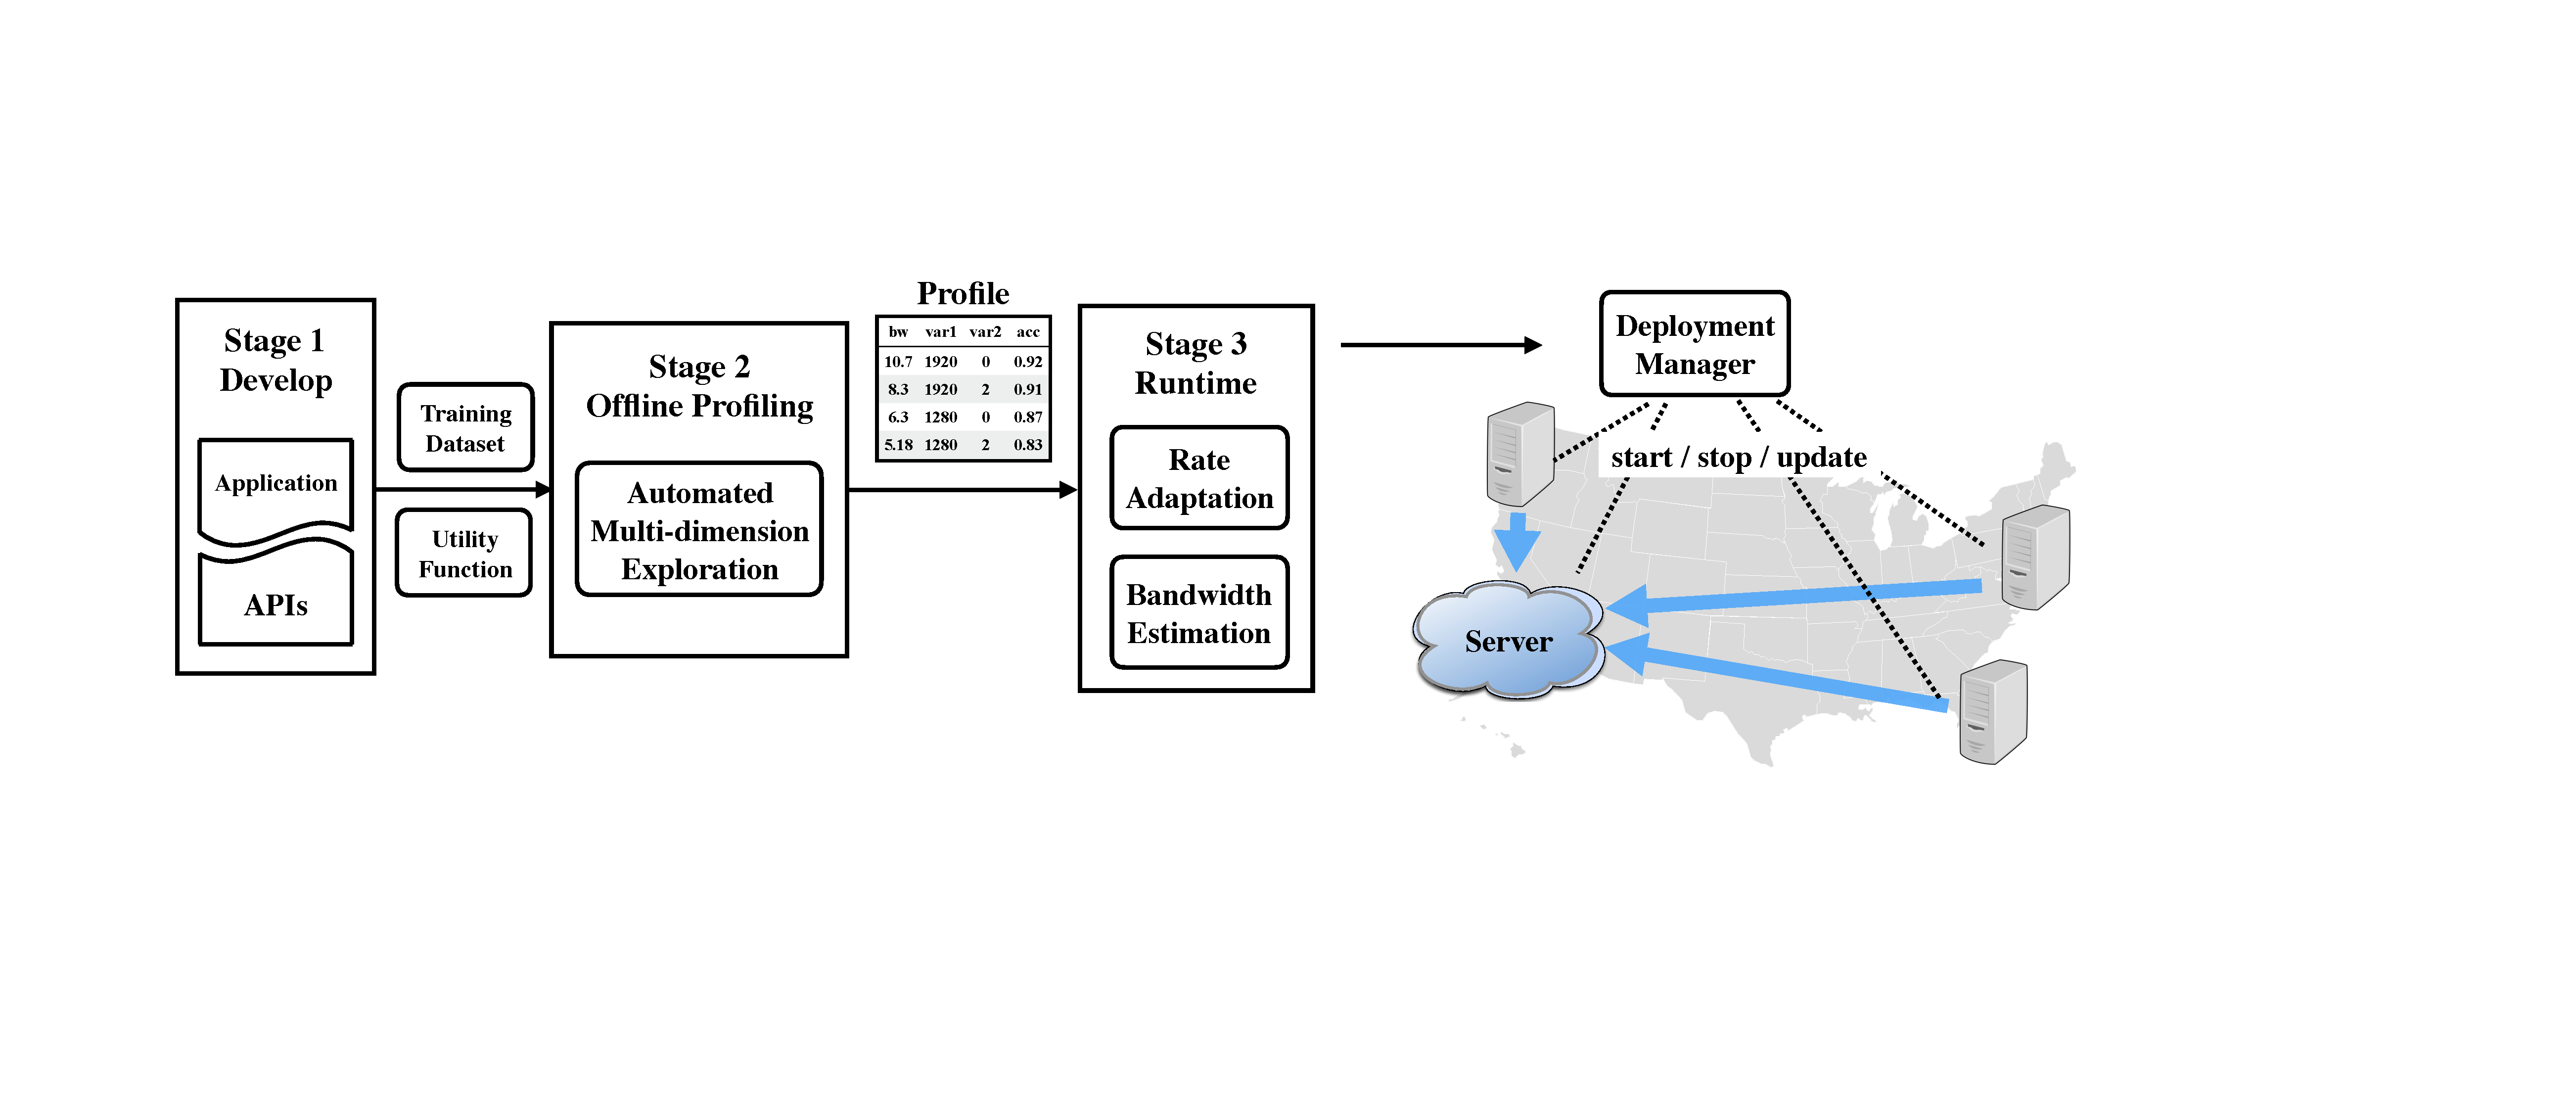
\includegraphics[width=\linewidth]{figures/arch.pdf}
  \caption{The three-stage architecture of \sysname{}.}
  \label{fig:overview}
\end{figure*}

To address the aforementioned challenges, \sysname{}'s solution is split into
three parts (\autoref{fig:overview} illustrates them).

\para{Programming abstraction~(\autoref{sec:prog-abs}):} Applications are
modelled as a directed acyclic graph (DAG) of computations. In addition to the
normal operators from existing systems, I propose a novel set of \texttt{maybe}
operators to express the specification of degradations. The proposed APIs do not
require developers to be exact on the quantity, making effort to integrate with
existing applications minimal.

\para{Automatic multi-dimensional profiling~(\autoref{sec:profiling}):} The
system automatically explores the parameter space to learn a Pareto-optimal
degradation strategy in a application-specific manner. This process frees
application developers from a tedious and repetitive process.

\para{Runtime Adaptation~(\autoref{sec:adaptation}):} Finally the streaming
application is deployed with a wide-area orchestration manager. At runtime,
\sysname{} provides all the necessary modules that act as the control plane and
adapt the application execution. At a high level, it performs bandwidth
estimation, congestion monitoring and adaptation. It uses the profile learned
from the second stage to guide the level of degradation.

\section{Programming Abstraction}
\label{sec:prog-abs}

Applications in \sysname{} are composed by connecting a set of operators to form
a dataflow graph. The system provides a basic set of APIs such as \texttt{map},
\texttt{filter}, \texttt{window} (\autoref{tab:operators}). The normal operators
are similar to existing stream processing systems; the core contribution of this
thesis is the set of \texttt{maybe} APIs that allows the specification of
degradation operations for bandwidth-accuracy trade-off.

\begin{table*}
  \small
  \centering
  \begin{tabular}{ c r l }
    \toprule
    \multirow{7}{*}{\begin{tabular}{@{}c@{}}Normal \\ Operators\end{tabular}}
    & \textit{map}(f: I $\Rightarrow$ O) & Stream<I> $\Rightarrow$ Stream<O> \\
    & \textit{filter}(f: I $\Rightarrow$ bool) & Stream<I> $\Rightarrow$
                                                 Stream<I> \\
    & \textit{skip}(i: Int) & Stream<I> $\Rightarrow$ Stream<I> \\
    & \textit{sliding\_window}(count: Int, f: Vec<I> $\Rightarrow$ O) & Stream<I> $\Rightarrow$
                                                                            Stream<O> \\
    & \textit{tumbling\_window}(count: Int, f: Vec<I> $\Rightarrow$ O) & Stream<I> $\Rightarrow$
                                                                             Stream<O> \\
    & \textit{timed\_window}(time: Duration, f: Vec<I> $\Rightarrow$ O) & Stream<I> $\Rightarrow$
                                                                          Stream<O> \\
    & ... & ... \\
    \midrule
    \multirow{4}{*}{\begin{tabular}{@{}c@{}}Degradation \\ Operators\end{tabular}}
    & \textit{maybe}(knobs: Vec<T>, f: (T, I) $\Rightarrow$ I) & Stream<I> $\Rightarrow$
                                                                 Stream<I> \\
    & \textit{maybe\_skip}(knobs: Vec<T>) & Stream<I> $\Rightarrow$ Stream<I> \\
    & \textit{maybe\_downsample}(knobs: Vec<(Int, Int)>) & Stream<Image> $\Rightarrow$ Stream<Image> \\
    & ... & ... \\
    \bottomrule
  \end{tabular}
  \caption{A comparison between normal stream processing operators and our
    degradation operators. Vec<T> represents a list of elements of type
    T. Notice the type constrain on the second argument passed to
    \texttt{maybe}.}
  \label{tab:operators}
\end{table*}

\subsection{Degradation Operators}
\label{sec:prog-abs}

To design the degradation operator, let's first consider a strawman solution:
manual policies for degradation. JetStream~\cite{rabkin2014aggregation} offers
an example: ``if bandwidth is insufficient, switch to sending images at 75\%
fidelity, then 50\% if there still isn't enough bandwidth. Beyond that point,
reduce the frame rate, but keep the images at 50\% fidelity.'' This manual
policy specification has the following issues:

\para{Lack of precision:} These policies are often developer heuristics and
rarely backed up by measurements. First, there is no direct association of the
application accuracy with the 75\% fidelity configuration. Besides, the effect
of each rule on the data size is not trivially available.  While it seems
intuitive that the level of degradation will change the data size, the precise
effect is not always straightforward. For example, one might think that reducing
the frame rate by 50\% will half the data rate. When video encoding is employed,
the inter-frame difference will increased (P-frame size) when the frame rate is
reduced. This leads to a larger data size for each frame. \autoref{fig:h264}
illustrates this complex relationship with an example of H.264 encoding under
four different frame rates.

\para{Not scalable:} The strawman solution quickly leads to too many policies
when multiple degradation operations are involved or a fine-grained control is
desired. This manual process becomes tedious and error-prone. When too few rules
are provided, the application may oscillate between two rules: one that's too
aggressive (always faces insufficient bandwidth) and one that's too conservative
(a suboptimal strategy).

\begin{figure}
  \centering
  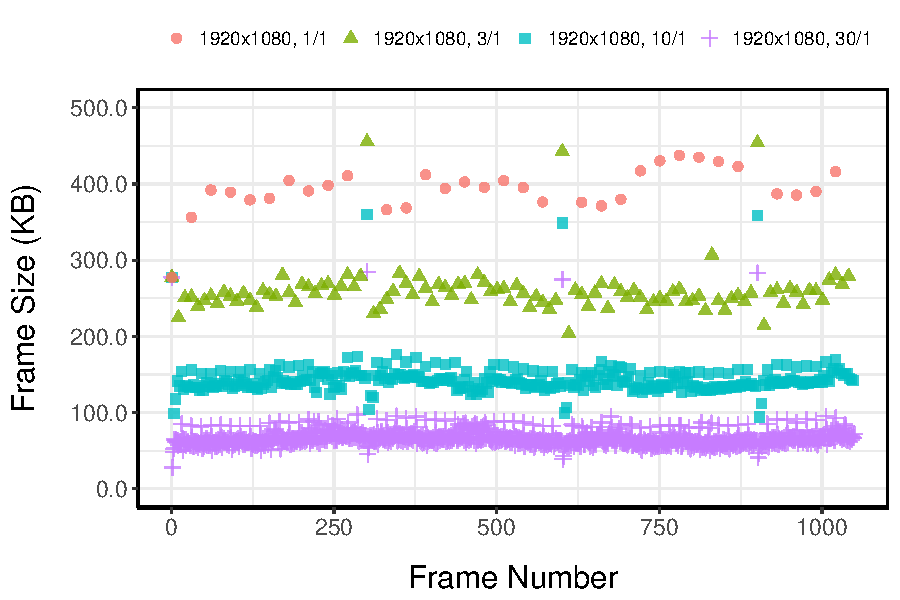
\includegraphics[width=\columnwidth]{figures/h264.pdf}
  \caption{H.264 requires more information per frame when the frame rate is
    reduced. All measurements are for videos with 1920x1080 resolution and the
    same H.264 configurations. 1/1, 3/1, 10/1 and 30/1 in the legend mean that
    the frame rates are 1 FPS, 3 FPS, 10 FPS and 30 FPS.}
  \label{fig:h264}
\end{figure}

\vspace{0.5em}

I argue that when using the above strawman solution, developers are forced to
manually study and measure the effect of individual degradation policy,
prohibiting its wide adoption in practice.

On the other extreme of the design spectrum lies a completely developer-free
solution. It is not practical, either. While static analysis has been shown to
optimize application execution adaptively in a mobile-cloud
context~\cite{chun2011clonecloud}, it only concerns with computation placement
(on the mobile or in the cloud) rather than tuning application parameters.  For
our dataflow programming model, static analysis is prone to false positives:
exploring wrong or unnecessary parameters. For example, when the application is
configured to generates statistics with a \texttt{timed\_window} operation,
static analysis may falsely detect the duration parameter and alter the behavior
of the application in an unexpected way. Also, as we will illustrate
in~\autoref{sec:profiling}, with each introduced parameter, the profiling time
increases drastically as all parameters pose a combinatorial space. The
explosion of search space prohibits explorations of unnecessary parameters.

\sysname{} takes a middle ground between these two extremes: developers use a
novel \texttt{maybe} API to annotate degradation operations without being exact
on the values. Think of these APIs as hints from developers: this operation,
when in use, will likely reduce the data size and affect the data fidelity;
however the exact quantity is not clear.

The basic form of \texttt{maybe} operator takes two arguments: a knob and a
degradation function (see \autoref{tab:operators}). The knob indicates different
degradation levels; the function performs the actual degradation operation with
a configurable level. There is one restriction on the type signature of the
function argument: $f(T, I) \Rightarrow I$. That is, the degradation function
should not alter the type of the stream. While this seems a strong restriction,
when combined with the \texttt{map} operator, the API set is still expressive
enough. I describe the implementation and usage of the APIs
in~\autoref{sec:implementation}.

Based on the \texttt{maybe} primitive, one can implement wrappers for common
degradation operations. For example, \texttt{maybe\_skip} will optionally
subsample a stream; \texttt{maybe\_downsample} can adjust the image resolution
to a configured target. Using the \texttt{maybe} API, the example mentioned
earlier can now be implemented as follows:

\begin{lstlisting}
   let app = Camera::new((1920, 1080, 30))
      .maybe_downsample(vec![(1600, 900), (1280, 720)])
      .maybe_skip(vec![2, 5])
      .map(|frame| frame.show())
      .compose();
\end{lstlisting}

This snippet first instantiates a \texttt{Camera} source, which has the type
\texttt{Stream<Image>}. It's configured to produce images with 1920x1080
resolution and 30 FPS. Two degradation operations are chained after the source:
one that downsamples the resolution to either 1600x900 or 1280x720; the other
skips frames with a parameter of 2 or 5, resulting in $30 / (2+1) = 10$ FPS or
$30/(5+1) = 5$ FPS. After the degradation, images are shown on the display; in
practice, further processing operators can be chained after the degradation.

While the API itself has simplified the specification of degradation, the exact
amount has to be known for precise rate adjustment at runtime. We then turn to
the second stage of our system that performs the automatic profiling.

\section{Multi-dimensional Profiling}
\label{sec:profiling}

The goal of this profiling stage is to explore the bandwidth-accuracy trade-off
and learn a Pareto-optimal \textit{profile} for a specific application and its
target scenario.

First, we define the terms and notations. Each \texttt{maybe} operator within an
application corresponds to a knob $k$. Suppose the application has $n$ knobs,
their combination forms a configuration $c = [k_{1}, k_{2}, ... k_{n}]$. The set
of all configurations $\mathbb{C}$ is the space that our profiling system need
to explore.

There are two mappings that we are interested: a mapping from a particular
configuration to its bandwidth requirement $B(c)$ and the accuracy measure
$A(c)$. The Pareto-optimal set $\mathbb{P}$ can then be defined
(\autoref{eq:pareto}): for all $c \in \mathbb{P}$, there is no alternative
configuration $c'$ that requires less bandwidth while giving a higher accuracy.

{\small
\begin{equation}
  \mathbb{P} = \{ c \in \mathbb{C} : \{ c' \in \mathbb{C}: B(c') < B(c),
  A(c') > A(c) \} = \varnothing\}
  \label{eq:pareto}
\end{equation}
}%

\begin{table}
  \centering
  \begin{tabular}{r l}
    \toprule
    \textbf{Symbol} & \textbf{Description} \\
    \midrule
    $n$ & number of degradation operations \\
    $k_i$ & the \textit{i}-th degradation knob \\
    $c = [k_{1}, k_{2}, ... k_{n}]$ & one specific configuration \\
    $\mathbb{C}$ & the set of all configurations \\
    \midrule
    $B(c)$ & bandwidth requirement for $c$ \\
    $A(c)$ & accuracy measure for $c$ \\
    $\mathbb{P}$ & Pareto efficienct set \\
    \bottomrule
  \end{tabular}
  \caption{Notations used in profiling.}
  \label{tab:notations}
\end{table}

Since there is often no closed form relation for $B(c)$ and $A(c)$, for
arbitrary degradation operations, \sysname{} takes a data-driven approach: with
a representative dataset and an application-specific utility function, the
system evaluates each configuration for their bandwidth demand and the
application utility. The utility could either be measured against the
groundtruth; or in the case when labelled dataset is not available, the system
uses the reference results when all degradations are turned off.

\begin{figure}
  \centering
  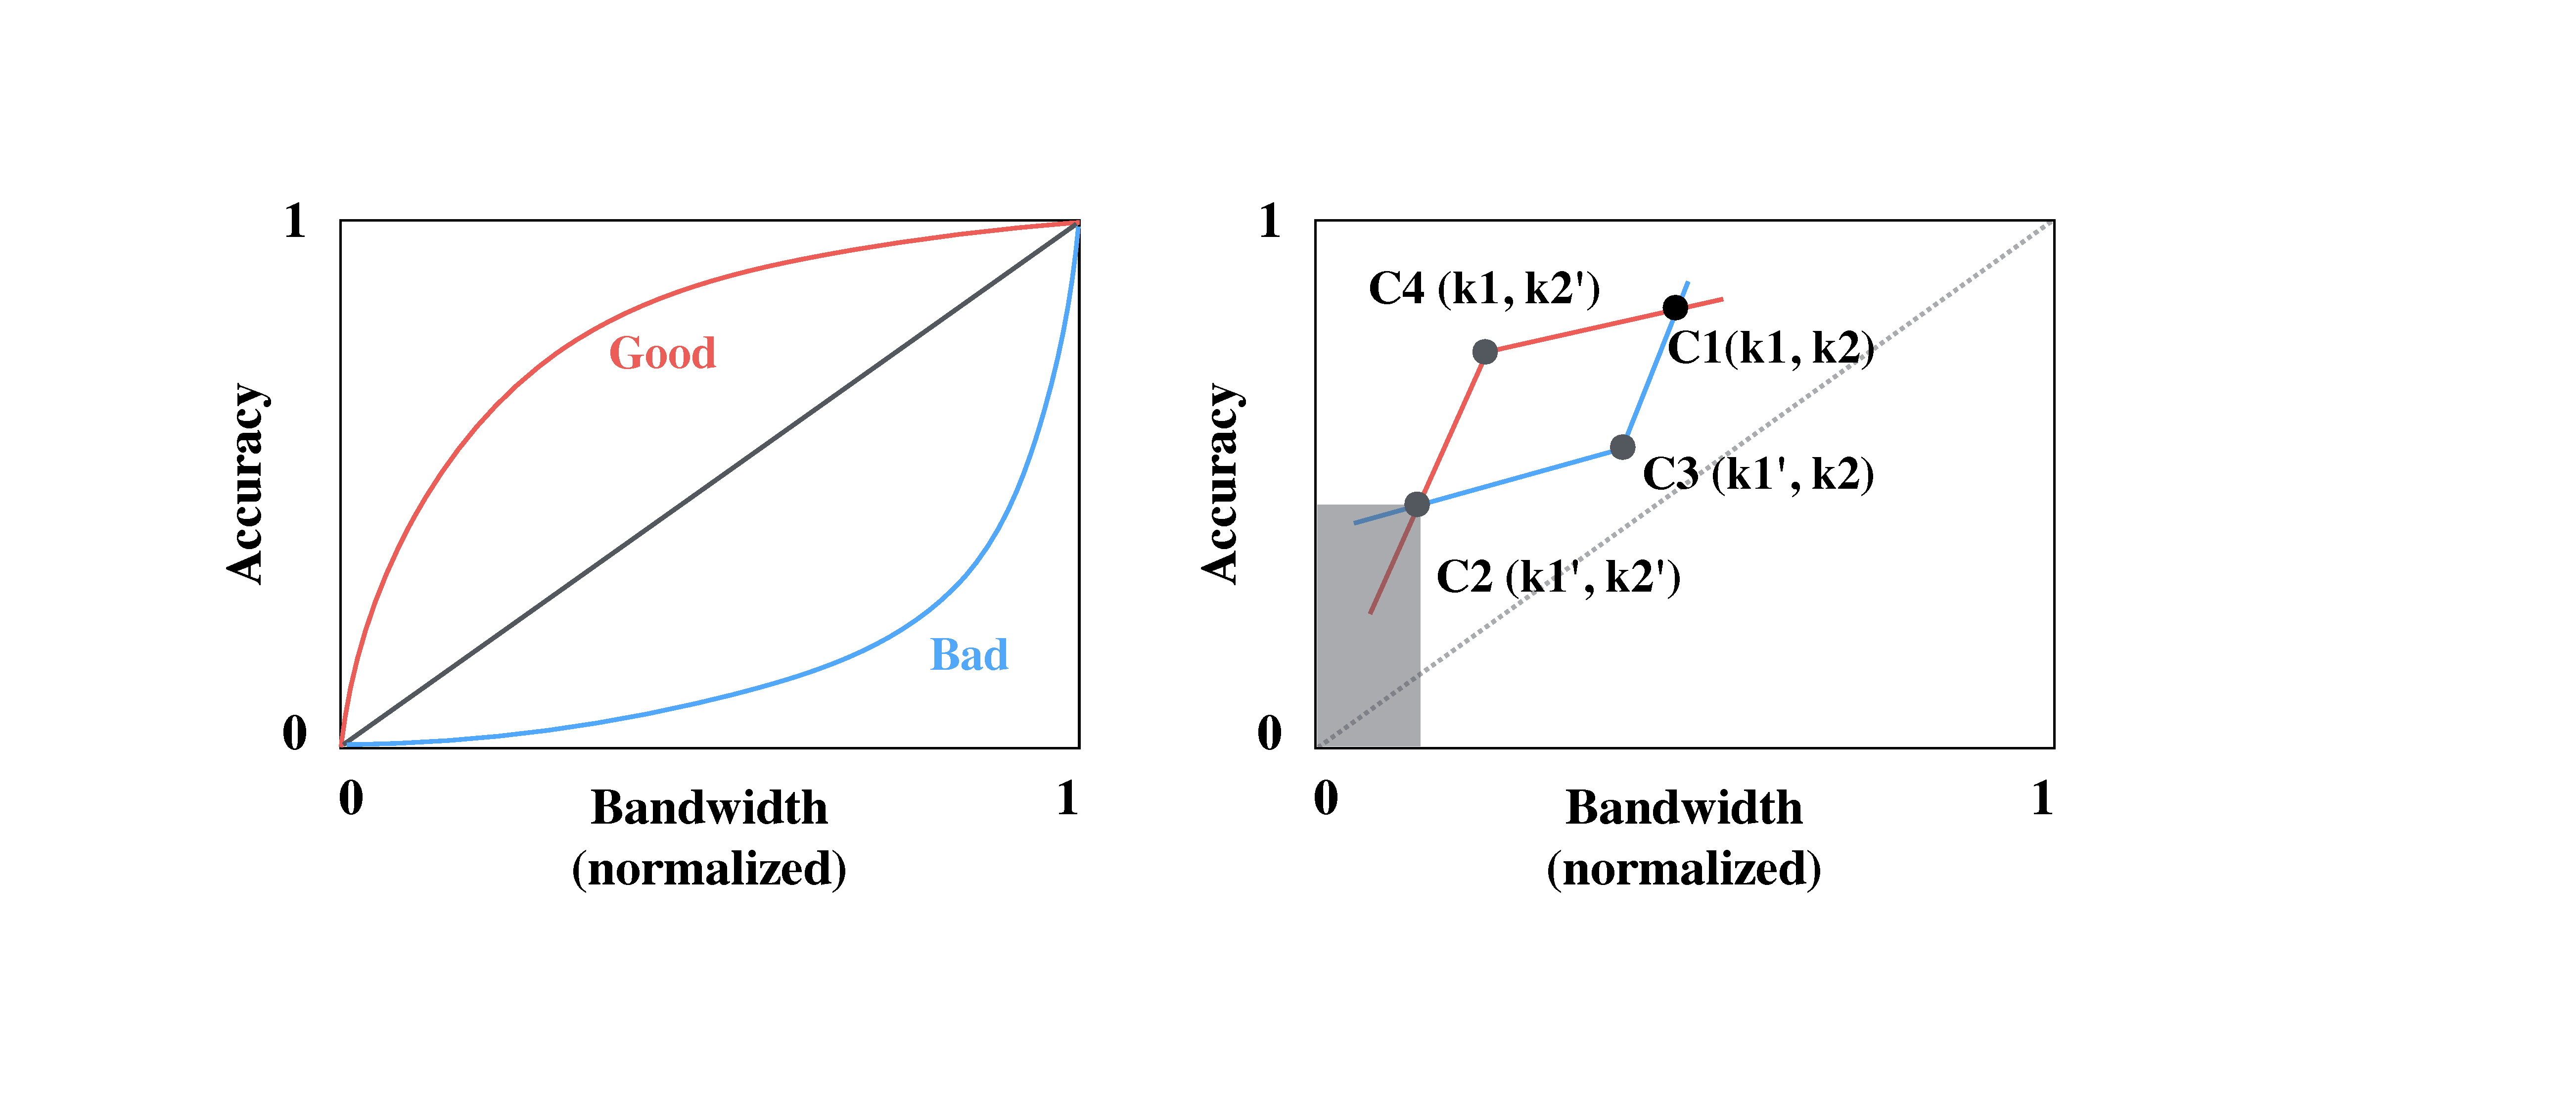
\includegraphics[width=\columnwidth]{figures/degrade.pdf}
  \caption{Illustration on the behavior of different degradation operations.}
  \label{fig:bat}
\end{figure}

When only one knob is involved, we can represent its impact using
bandwidth-accuracy curve (\autoref{fig:bat} left). The point on the curve has a
coordinate $(B(c), A(c))$ when configuration $c$ is used. The straight line from
(0, 0) to (1, 1) splits the space into two parts. Along this line, the amount of
bandwidth saving leads to an equal amount of accuracy drop (when both quantity
normalized to 1). If a degradation's profile lies above this line, it indicates
an effective degradation that should be employed as it offers little accuracy
drop with more bandwidth savings. For degradation operations below the straight
line, data information loss is more severe than the savings when the degradation
is in effect. One quantity to capture the relative power of different
degradation strategy is to use the area under the curve (AUC). With this setup,
the Pareto-optimal strategy can be define as the curve that has a maximal AUC.
We will show a few concrete profile curves in~\autoref{sec:evaluation}.

While $B(c)$ and $A(c)$ are usually monotonic along individual dimension $k_i$,
when multiple degradations combined, each curve may have a distinct shape. The
right side of \autoref{fig:bat} illustrates this complex
relationship. \todo{write more}.

Although the complexity of degradation operations prohibits further
optimizations to reduce the profiling time, there are several techniques in
practice that can make the problem tractable: (i) Exploring these configurations
is an offline task; there is no direct dependencies among configurations,
resulting in an embarrassingly parallel task. Executed in a cluster, it scales
out perfectly with provided compute resources. (ii) When the degradation level
increases or when multiple degradation operations are in effect, the amount of
data to be analyzed becomes smaller; also the computational complexity for each
data item can also be dramatically reduced. (iii) Developers can specify a lower
bound on the accuracy and the profiling can stop exploring worse configurations.
Once there is a known configuration that is worse than the configured threshold,
configurations with a larger level of degradation do not need to be profiled
(such as the gray area in \autoref{fig:bat}).

\section{Runtime Adaptation}
\label{sec:adaptation}

\begin{figure}
  \centering
  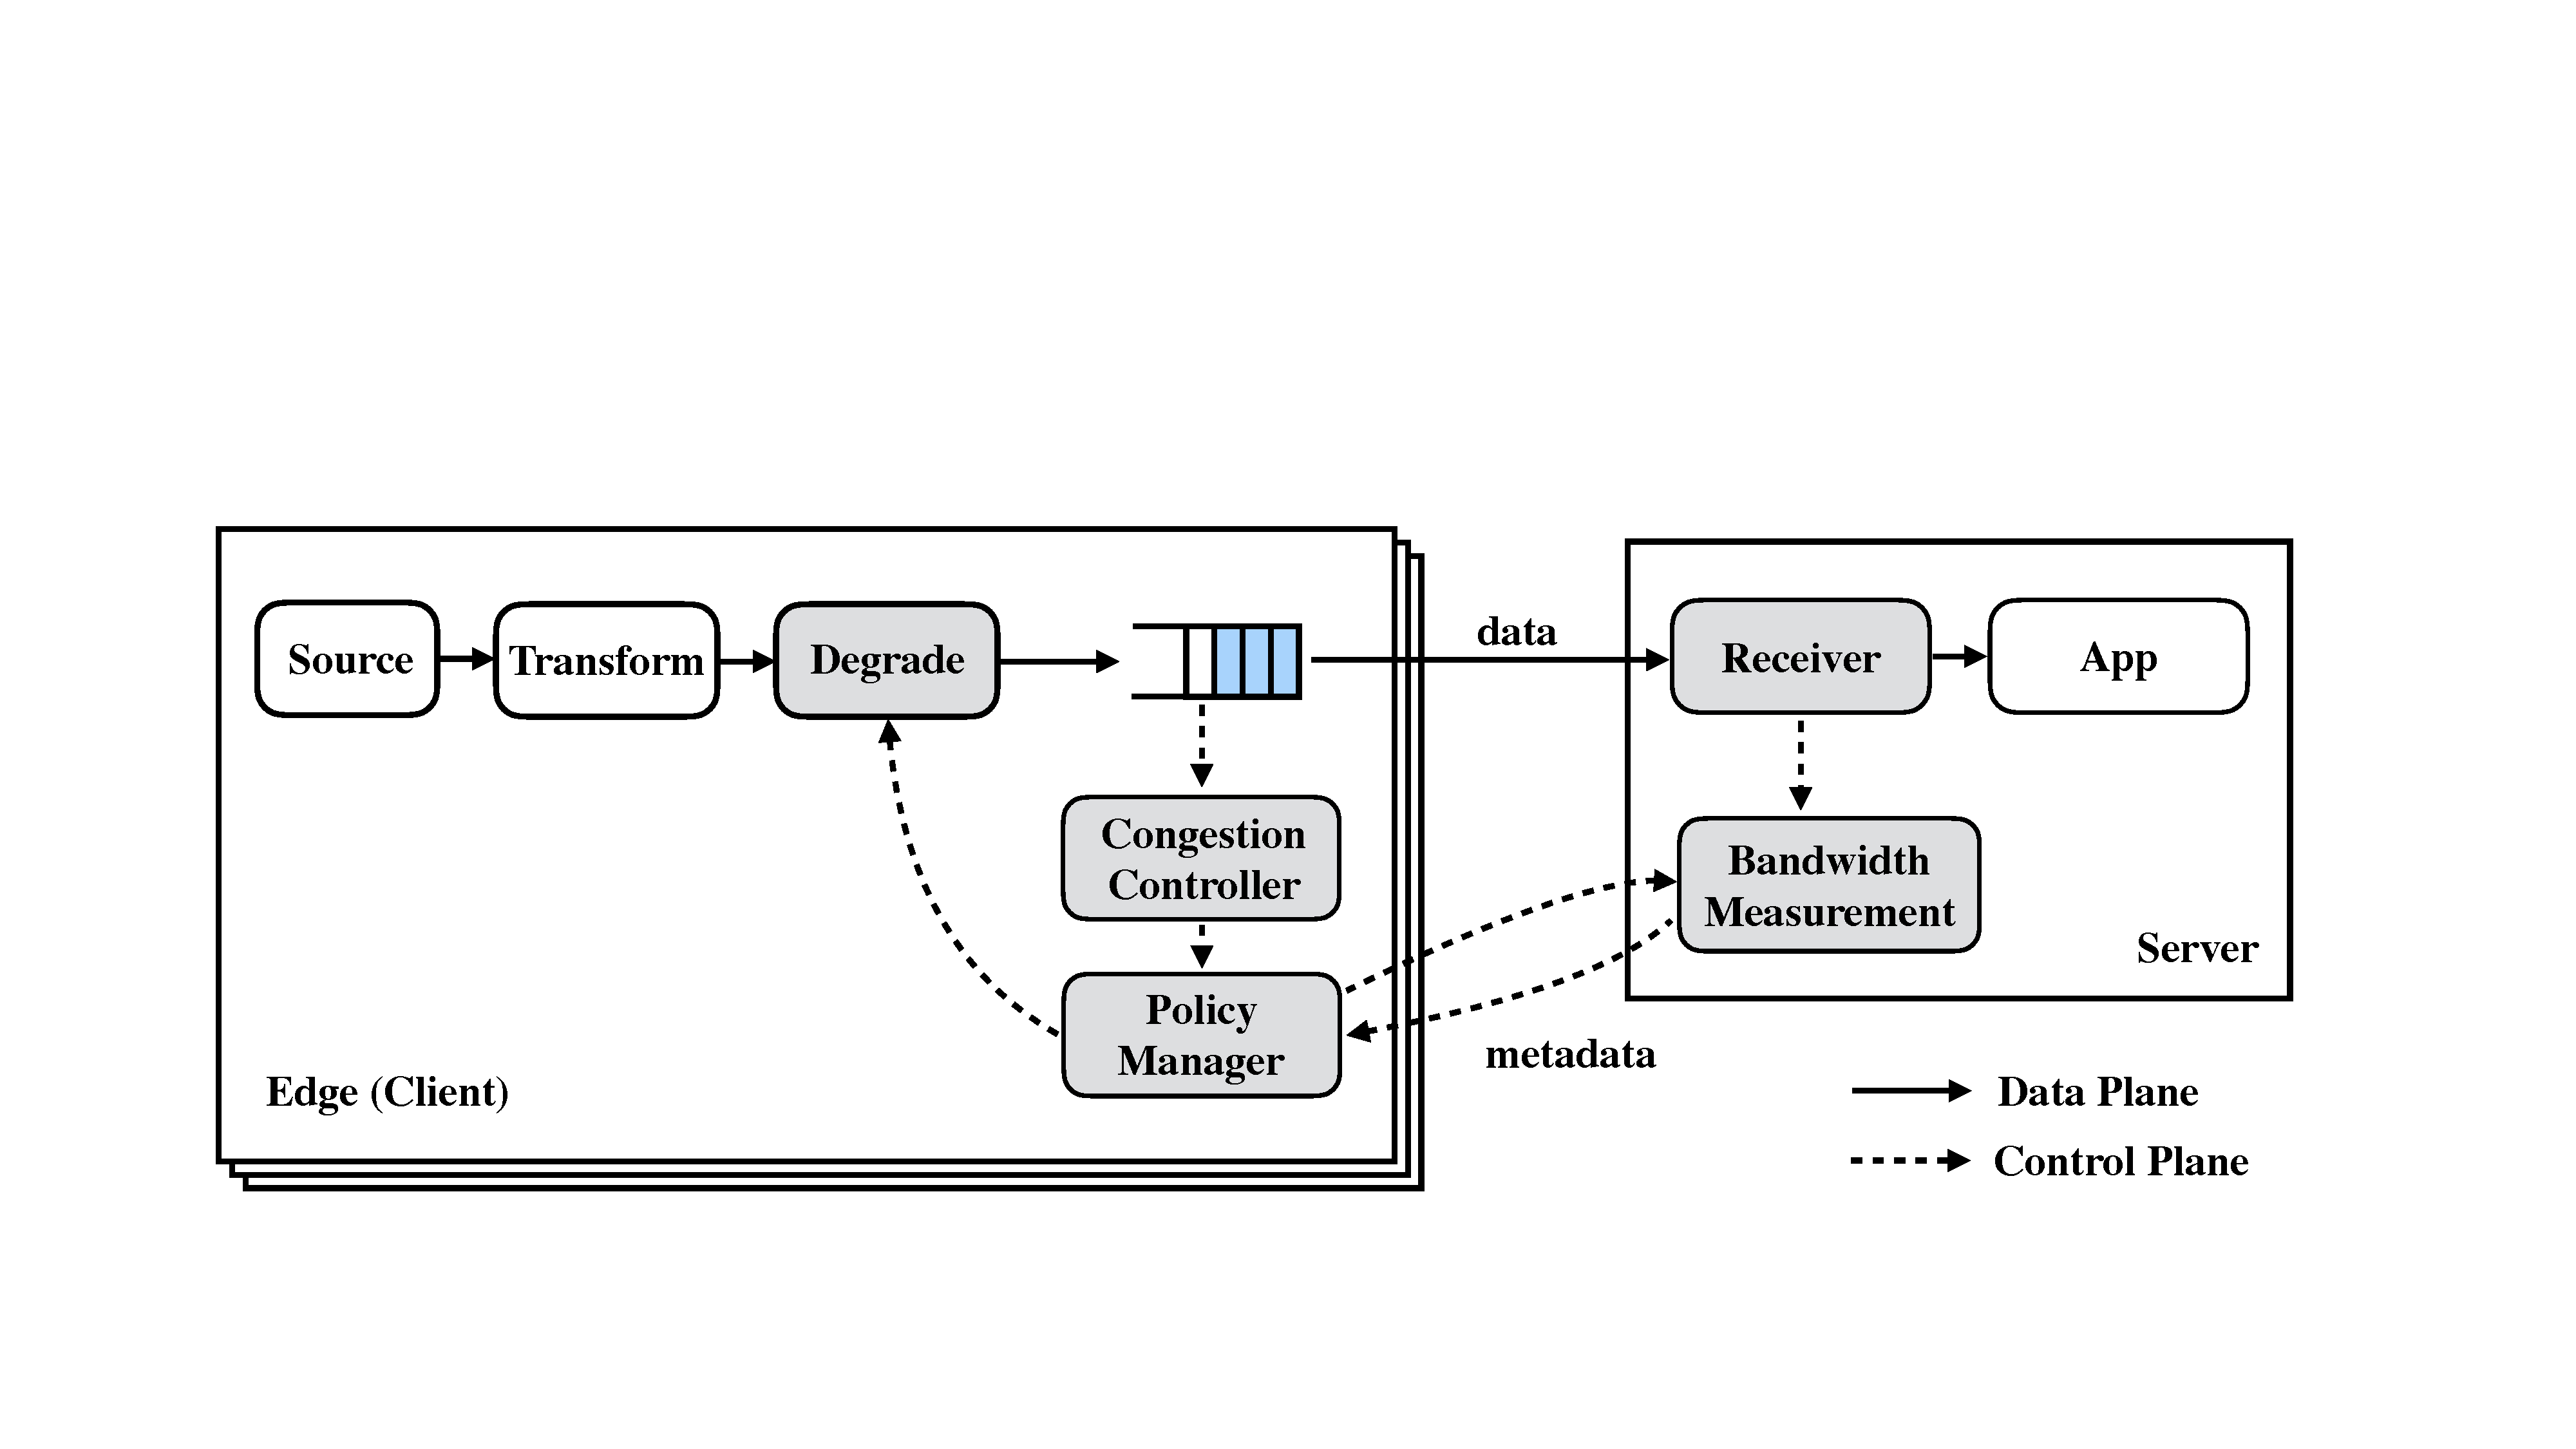
\includegraphics[width=\linewidth]{figures/runtime.pdf}
  \caption{Runtime adaptation system architecture. \sysname{}'s provided
    components are grey: they form the control plane to compensate the
    application's data plane.}
  \label{fig:runtime}
\end{figure}

\todo{stop here.} At runtime, the user program is automatically converted to a
client half and server half; and \sysname{} abstracts the communication as well
as rate adaptation. \autoref{fig:runtime} shows our runtime architecture.

\para{Object-level queue:} The queue bridges data generation and
the network capacity. It transmits data as fast as the network can handle and
detects congestion when the queue grows.

\para{Congestion controller:} Our first prototype used the queue length as a
signal for congestions, this turns out to be a bad match as the degradation
operation may change object arrival rate (e.g.\,lower frame rate for video). Our
next version uses data size, but it also leads to long latency when the
degradation changes individual object size (e.g.\,lower resolution). Our current
design uses an adaptive size: given current configuration and the profile, the
queue learns the desired data generation rate (bps), and with a user configured
latency, the queue derive the congestion watermark.

\para{Bandwidth Measurement:} The receiver delivers the received data to
application. In the meantime, it measures the effective throughput between each
client-server pair as an indication of current bandwidth~\cite{iperf}. To avoid
spikes in the bandwidth measurement, exponential smoothing is employed. While
the receiver performs bandwidth measurement every second, it does not send the
information back to each client.  avoid unnecessary communication, the client
requests the measurement only when congestion is detected.

\para{Policy Manager:} Upon receiving signals from congestion controller, it
performs an RPC request to the server for current bandwidth measurement. With
the learned profile, it determines the degradation level and start the actual
degradation strategy. The bandwidth specification in the learned profile is the
required bandwidth, the policy manager usually takes a conservative approach:
using a constant rate ALPHA to adjust the available bandwidth. When the
congestion is resolved, the policy manager gradually reduce the degradation
level (additive increase phase).

\para{Degrade:} The actual degradation operation is rather simple. Operators
based on the \texttt{maybe} API supports a \texttt{set} function that would
change the internals of the operator. The \texttt{set} function is invoked when
degradation is needed.

%% {Interaction with TCP:} Our runtime system follow the tuning guide
%% \cite{tierney2001tcp} to adjust the send buffer.

%%% Local Variables:
%%% mode: latex
%%% TeX-master: "sigcomm2017"
%%% End:

%%% Local Variables:
%%% mode: latex
%%% TeX-master: "thesis"
%%% End:

\chapter{Implementation}
\label{sec:implementation}

In this section we present details about our implementation, including a
prototype framework and three non-trivial wide-area streaming applications.
\sysname{} is implemented in Rust and open-source on Github.\footnote{Url elided
  for anonymity.}

\section{Framework}
\label{sec:framework}

While our proposed APIs are general and not language specific, we chose a safe
language, Rust, for the core framework for the following reasons. First, Rust's
memory safety guarantee can ensure applications running continously for an
extended period of time. Besides, the zero-cost abstraction removes the
possibilities of tail latencies caused by uncoordinated garbage
collection~\cite{maas2016taurus}. In addition, we rely on Rust's type system to
enforce the type match on \texttt{maybe} operations.

\begin{sloppypar}
All operators implement the \texttt{Stream} trait which has an associate type
\texttt{Item} and a core function \texttt{next} that returns
\texttt{Datum}. Each datum is either an item with the \texttt{Stream::Item} or
an \texttt{Error} that the operator use to communicate with the runtime
scheduler. The concrete form of \texttt{maybe} API is almost an direct
translation of the API specification. While our API specification
in~\autoref{tab:operators} uses a vector for knobs, our Rust implementation is
more general: any type (including vector) that implements \texttt{IntoKnob}
trait can be used as the knob.
\end{sloppypar}

\begin{lstlisting}
pub trait Stream {
    type Item;
    fn next(&mut self) -> Datum<Self::Item, Error>;

    fn maybe<K, F>(self, opts: K, f: F) -> Maybe<Self, F>
        where Self: Sized,
                K: IntoKnob,
                F: FnMut(K::Item, Self::Item) -> Self::Item {

         // omitted
    }
}

pub trait IntoKnob {
    fn into_knob(self) -> Knob;
}
\end{lstlisting}

Developers can directly use the above API with user-defined functions. The
snippet below shows how a quantization degradation can be implemented with our
API. First, a vector of values is converted into a stream object. Then a
\texttt{maybe} operator with a knob value (2 or 3) and a function that performs
an interger division (quantization). Function \texttt{collect} will run this
stream and hold the output in a vector. Depending on the degradation level, the
output stream could either be [1, 2, 3, 4], [0, 1, 1, 2], or [0, 0, 1, 1].

\begin{lstlisting}
let quantized_stream = vec![1, 2, 3, 4]
    .into_stream()
    .maybe(vec![2, 3], |knob, p| p / knob);
    .collect();
\end{lstlisting}

We've also extended the basic API for common operations. As we are building
video processing applications, we implemented a specialized
\texttt{maybe\_downsample} operator can that wraps \texttt{downsample} function
internally.

\begin{lstlisting}
fn downsample(res: (usize, usize), image: Mat) -> Mat {

    //  omitted

}
\end{lstlisting}

Applications built with \sysname{} runs as a single process. The entire
processing pipeline is often specified in a single main file. The execution mode
(profiling, runtime as client or runtime as server) is configured with command
line arguments or environment variables. Our deployment manager is currently a
shell script using Docker container.

\section{Building \sysname{} Applications}
\label{sec:build-appl}

Using \sysname{}, we've built three applications: pedestrian detection
surveillance, an augmented reality and a distributed Top-k (\autoref{fig:apps}).
\autoref{tab:apps} summarizes the application specific part: knobs, utility
function and dataset

\begin{table*}
  \small
  \centering
  \begin{tabular}{|c|c|c|c|}
    \hline
    Application & Knobs & Utility & Dataset \\
    \hline
    Pedestrian Detection & resolution, framerate, quantizer
                        & F1 score & MOT16-04 (training), MOT16-03 (testing) \\
    \hline
    Augmented Reality & resolution, framerate, quantizer
                        & F1 score & Video clips of office (training), home (testing) \\
    \hline
    Top-K & head (N), local threshold (T) & Kendall's W & sec.gov access log
                                                          (4 days training, 12 days testing)  \\
    \hline
  \end{tabular}
  \caption{\sysname{} Applications}
  \label{tab:apps}
\end{table*}

\begin{figure*}
  \centering
  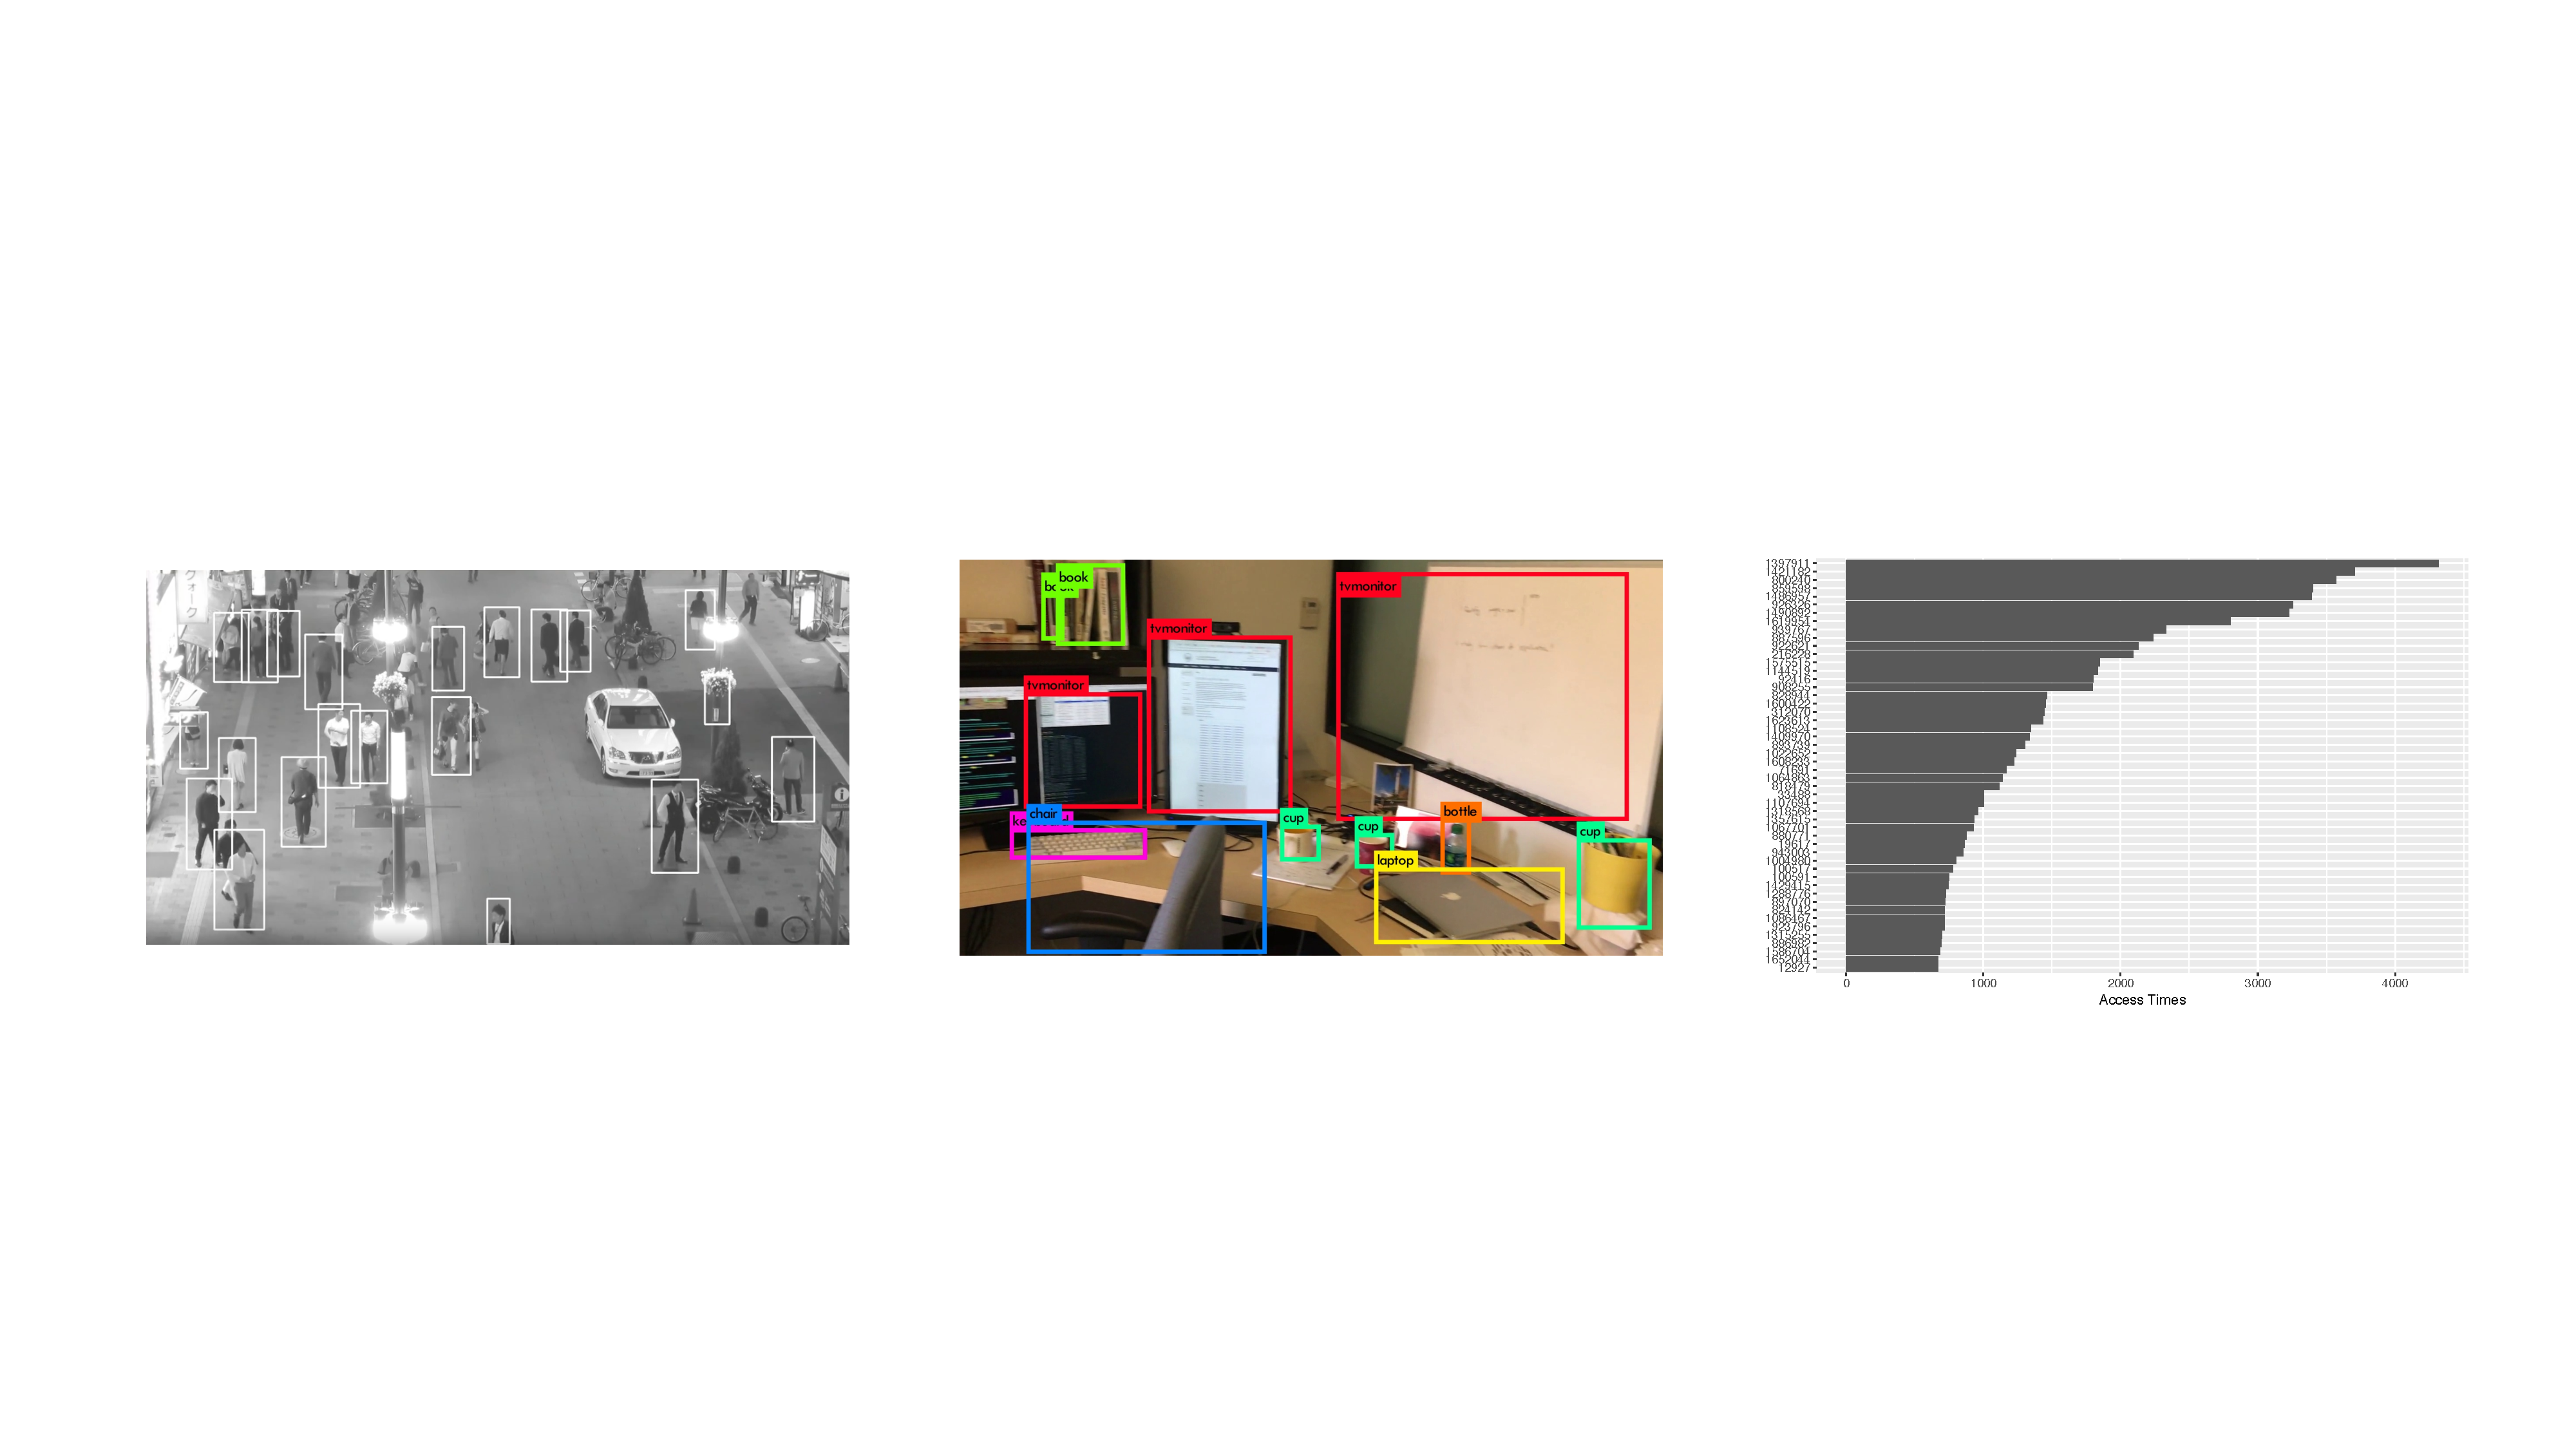
\includegraphics[width=.95\textwidth]{figures/apps.pdf}
  \caption{\sysname{} applications}
  \label{fig:apps}
\end{figure*}

\para{Pedestrian Detection:} This application analyzes video streams from
installed CCTV cameras and detect pedestrians inside. The detection result is a
list of bounding boxes representing pedestrian's relative location within the
view. Variant of this application can be used for safety monitoring, anomaly
detection or waiting line counting.

We implement most image-related operations with OpenCV
3.1~\cite{opencvlibrary}. Pedestrians are detected using histogram of oriented
gradients (HOG)~\cite{dalal2005histograms} with the default linear SVM
classifier. To ensure real-time processing of frames, GPU-accelerated
implementation is used in favor of the CPU-based implementation.

For video encoding, H.264 scheme is chosen for its prevalence in existing
systems. Our implemenation is based on GStreamer~\cite{gstreamer}, using
\texttt{x264enc} plugin. To integrate with \sysname{}, we first create a
pipeline that exposes \texttt{appsrc} (to feed raw image data) and
\texttt{appsink} (to get encoded bytes). The GStreamer main loop is managed in a
separate thread and \sysname{} communicates with it via Rust's channel. The
\texttt{x264enc} is configured with \texttt{zerolatency} present and runs using
four threads. It uses constant quality encoding and the quantizer is exported as
a parameter that can be tuned.

This application has three degradation operations: reducing image resolution,
dropping frame rate or lower video encoding quality.

The detection returns a list of bounding boxes; it's compared against a
reference result (either the groundtruth or the one without degradation). A
successful detection is defined when the intersection over union (IOU) is
greater than 50\%~\cite{everingham2010pascal}. For the utility function, we use
F1 score (\%), the harmonic mean of precision and
recall~\cite{Rijsbergen:1979:IR:539927}.

\para{Augmented Reality:} We target at mobile augmented reality applications
which offload the heavy computation to resources elsewhere. Although local
computation is gaining attraction~\cite{satyanarayanan2009case, zhang2015cloud},
wireless communication link is also susceptible to capacity variation.

We use a similar setup as the pedestrian detection application except the actual
function that analyzes the stream. To recognize objects, we use a a pre-trained
neural network~\cite{darknet13} that's trained with
Imagenet~\cite{krizhevsky2012imagenet}. Similar to our first application,
GPU-accelerated implementation is use in favor for real-time processing.

The utility function here is more strict than the pedestrian detection:
true-positive depends not only on IOU criteria, but also on the type of objects
(a correct identification).

\para{Distributed Top-K:} Many distributed system monitoring applications
require to answer the ``top-k'' question~\cite{babcock2003distributed}, such as
the top-k most popular URLs or the top-k most access files. Naive methods of
transmitting all the raw log entries to the aggregation point is not feasible as
popular servers typically have millions of requests per second. Local worker
node can first perform a window-based transformation that generates data
summary, such as key-value pairs of \texttt{<item, count>}. However, even after
this operation, the data size could still be too large given most real-world
access patterns follow a long-tailed distribution. There is a
large-but-irrelevant tail that is unnecessary to send.

We consider two degradation operations that individual worker nodes can perform:
(1) a local Top-\texttt{N} operation that shortens the list first; (2) a local
threshold \texttt{T} that further filters small entries. Obviously, these two
operations are not orthognal to each other. Their impact on data size reduction
and quality degradation depends on the distribution of the actual data.

\begin{figure}
  \centering
  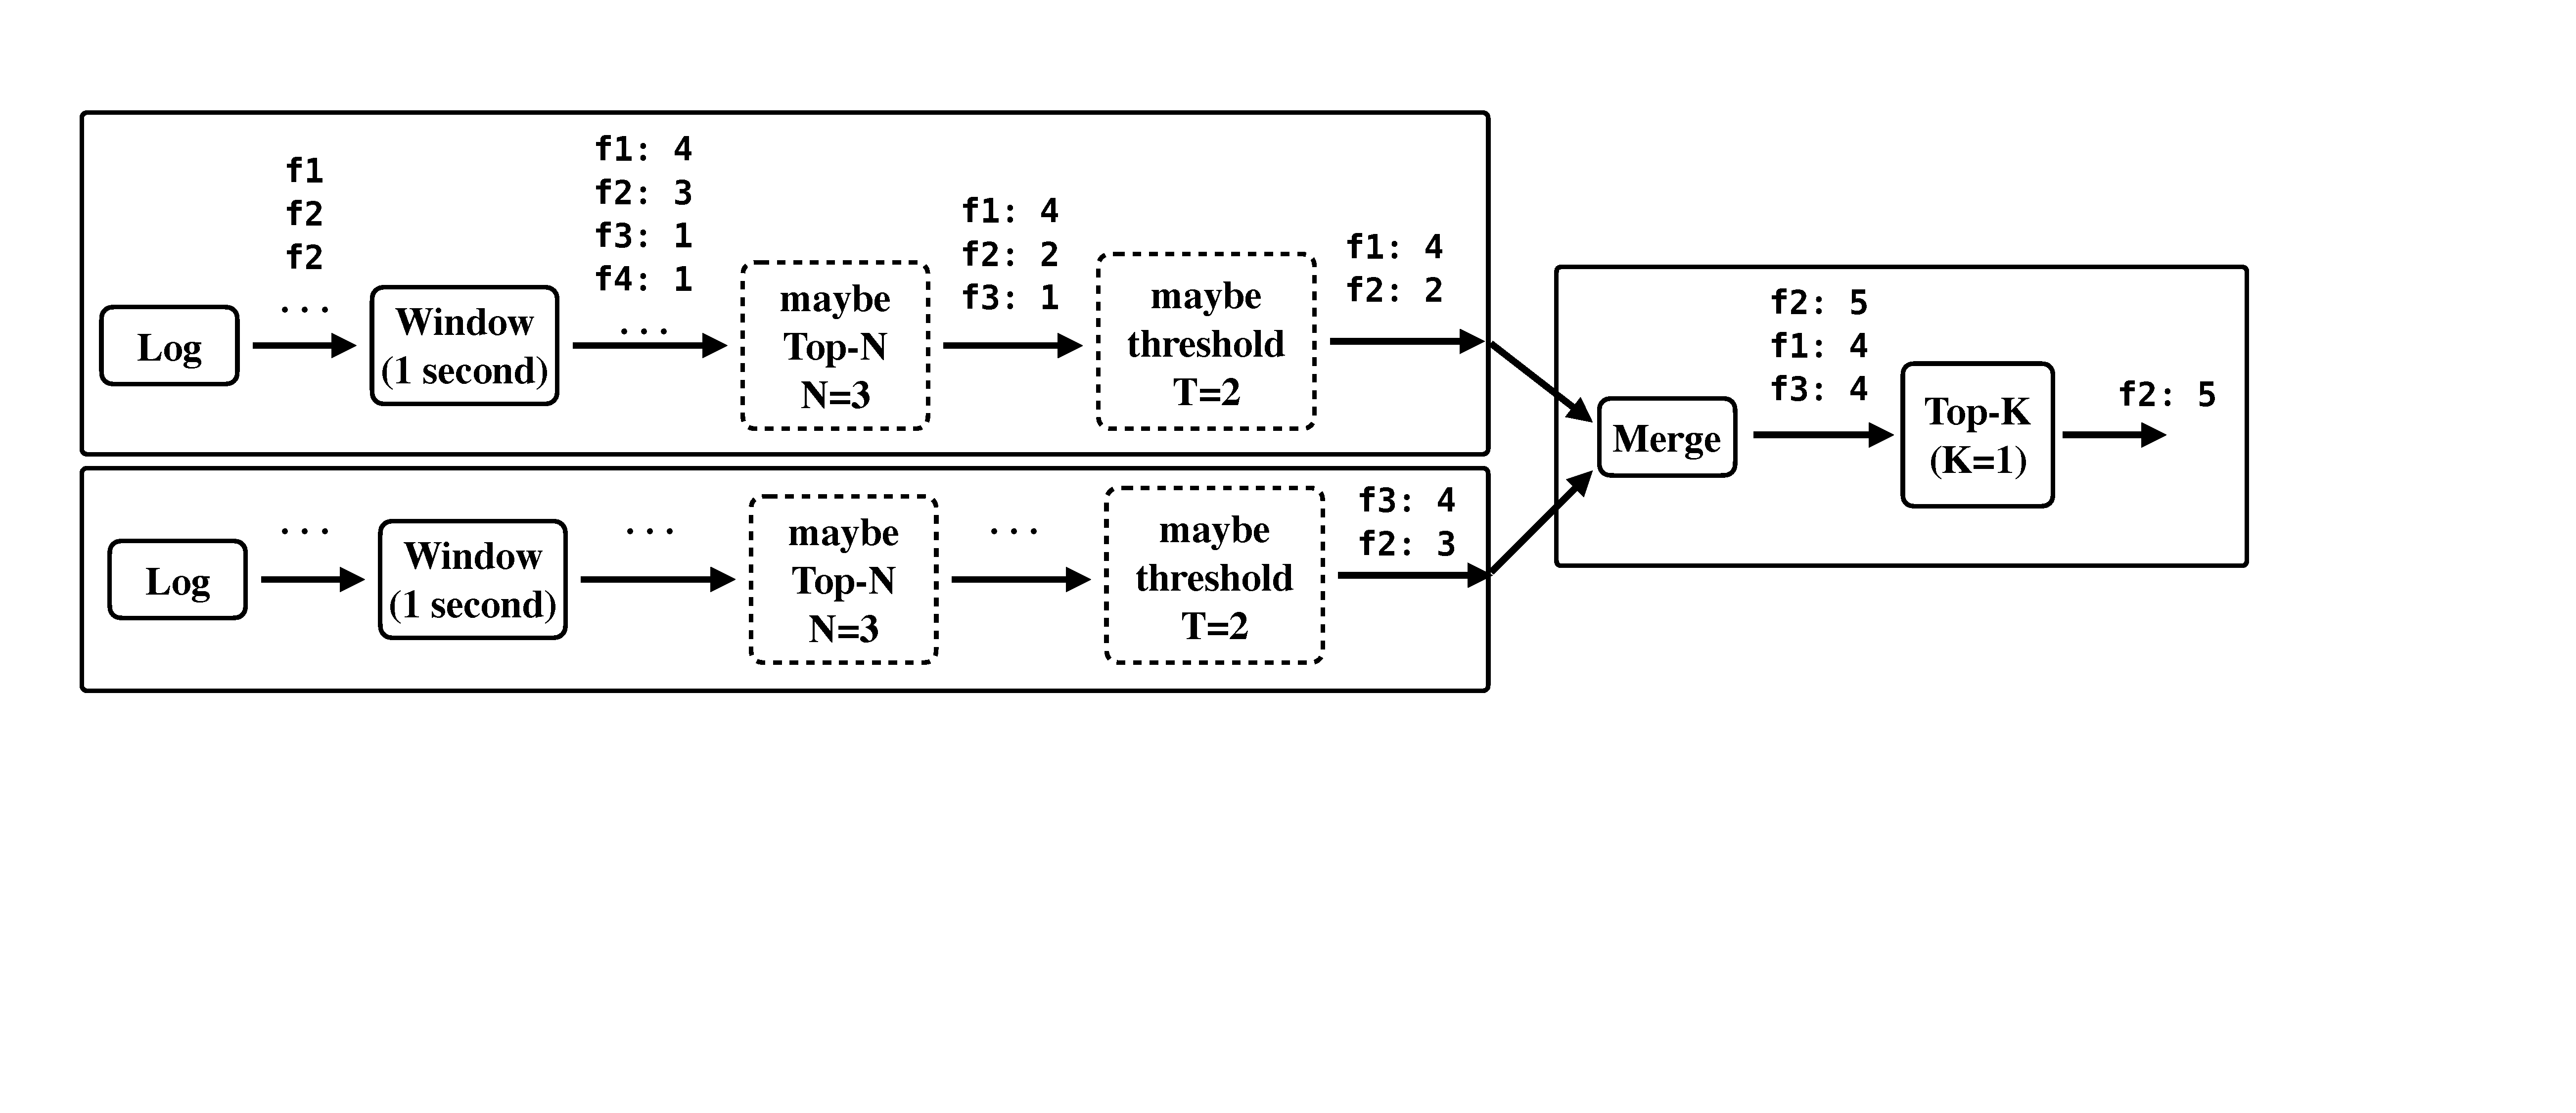
\includegraphics[width=\linewidth]{figures/topk.pdf}
  \caption{A distributed Top-K application has two tunable parameters: a local
    Top-N (N) and a local threshold (T).}
  \label{fig:topk}
\end{figure}


we use Kendall's W as the utility function here. It is a distance measure of the
concordance between two ranked list. The function outputs a statistic measure
ranging from 0 to 1, representing no agreement to complete aggrement,
respectively~\cite{abdi2007kendall}.


\section{Evaluation}
\label{sec:evaluation}

We first show the generated profile for the three applications. Then for each
application, We show how they adapt the behavior at runtime. Under a controlled
experiment, even with only transient network capacity drop, our system is able
to maintain an end-to-end delay for 10 seconds in the wide-area and accuracy
level above 80\%. Application-agnostic protocols creates significant backlogged
data (TCP for about 100 seconds) or unusable accuracy (UDP).

\subsection{Degradation Performance}
\label{sec:degr-perf}

\begin{figure}
  \centering
  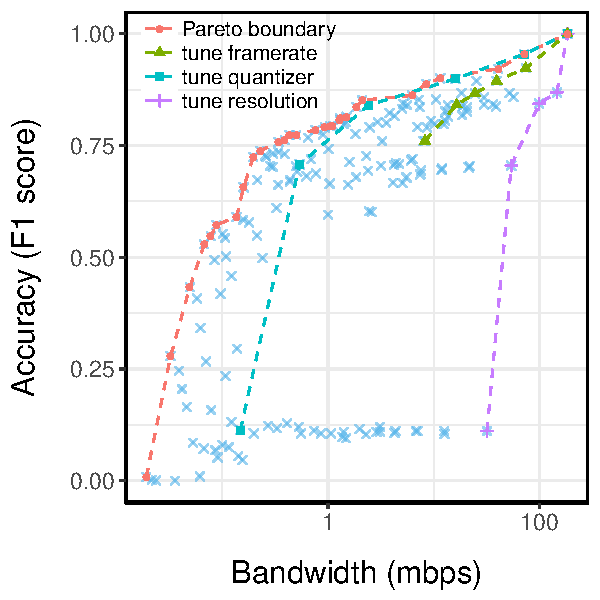
\includegraphics[width=0.6\textwidth]{figures/ped-profile.pdf}
  \caption{Pedestrian Detection}
  \label{fig:pd-profile}
\end{figure}

\begin{figure}
  \centering
  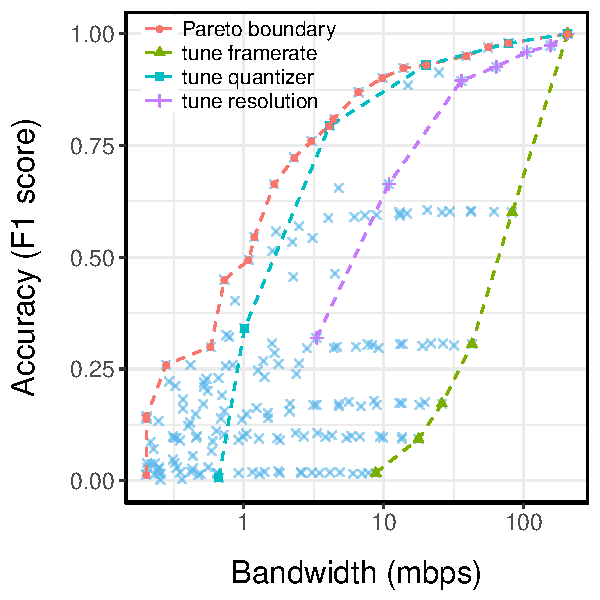
\includegraphics[width=0.6\textwidth]{figures/darknet-profile.pdf}
  \caption{Augmented Reality}
  \label{fig:ar-profile}
\end{figure}

\begin{figure}
  \centering
  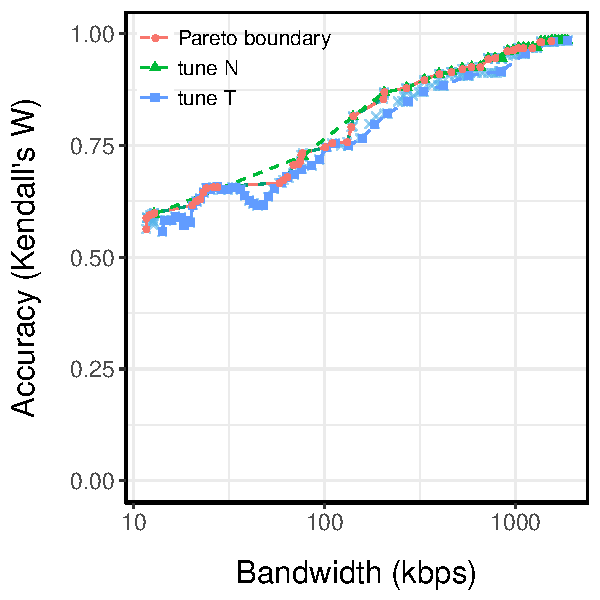
\includegraphics[width=0.6\textwidth]{figures/log-profile.pdf}
  \caption{Top-k}
  \label{fig:tk-profile}
\end{figure}

We describe the dataset we used for offline profiling and interpret the
profiling results (\autoref{fig:all-profiles}) in turn.

\para{Pedestrian Detection:} We use MOT16 dataset~\cite{milan2016mot16} to
evaluate this application. Specifically we used MOT16-04 as the training
dataset. The video feeds capture a busy pedestrian street at night with an
elevated viewpoint. The original resolution is 1920x1080, with frame rate
30. The training data has 1050 frames in total, amounting 35-second monitoring.
On averge there are 45.3 people per frame.

There are three knobs in this application: resolution, frame rate and encoding
quality. To maintain the same 16:9 aspect ratio with the original 1920x1080
resolution, the first degradation only chooses common 16:9 resolutions:
1600x900, 1280x720, 960x540, 640x320. For the framerate, integer values are
chosen in favor of fraction values. The original frame rate is 30, and our
degradation explores 10, 5, 3, 2, 1. H.264 encoding quantizer has a range from 0
(lossless) to 51 (worst possible), and 18 is the visually
lossless~\cite{bellard2012ffmpeg}. In our experiment, we use 10, 20, 30, 40, 50
as degradation parameters.

The generated profile is shown in~\autoref{fig:pd-profile} with x-axis the
required bandwidth and the y-axis the accuracy (F1 score). Note the log scale on
the horizontal axis as raw uncompressed 8-bit RGB video streams are
prohibitively large: $1920 \times 1080 \times 30 \times 3 \times 8 = 1.5 $ Gbps.

Each point in the scatter plot represents one configuration that our offline
profiling has evaluated. Notice the vast spread in bandwidth requirement among
configurations with similar accuracy as well as the wide spread in accuracy
among configurations that consumes similar bandwidth.

We first show three lines in the case of only tuning one knob. Notice the
distinct behavior of the three lines. In this particular application, reducing
the resolution has the most penalty because the HOG detector has a minimal 128
pixels by 64 pixels window. The camera is deployed in a far-field context;
scaling down the image will quickly has an effect on the detection. Tuning frame
rate doesn't affect the accuracy too much. In fact, even with 1 FPS, the
accuracy is still relatively high. However, reducing frame rate doesn't bring
much bandwidth saving (as we have mentioned in \autoref{fig:h264}).  The most
effective way that reduces the bandwidth while preserving the accuracy is to
adjust the quantizer because it affects almost every pixel and creates smaller
P-frames.

The Pareto boundary, or \textit{profile}, is the most important curve. In the
begining it's close to the curve when only quantizer is tuned, quantizer has a
certain limit. A crisp image is prefered as many image processing algorithms are
looking for the edges while for human consumption, a smoother image is fine.

As the uncompressed video is not practical, we imposes a bandwidth cap before
the profile is used in runtime (only use optimal configurations that creates
video with less than 20mbps data rate).

\para{Augmented Reality:} We collected training set for this application
ourselves. It's a 23-second video clip with 1920x1080 resolution and 30 FPS
taken on a mobile phone. During the capture, we change the camera view in a slow
pace to emulate how a real user would look around. Because target objects are
relatively close while the camera is moving, we hypothesis for this training
set, the profile will be different from the previous application that reducing
frame rate will have a detrimental effect.

The generate profile is shown in \autoref{fig:ar-profile}. First, we see our
intuition backed up by measurements. Besides, the Pareto boundary also first
follows the video encoding knob, but optimal settings are achieved only when
multiple degradations are in effect.

\para{Top-K:} To evalute the top-k application, we generate synthetic dataset
based on real-world access logs (EDGAR log file dataset, the access log of
\url{https://sec.gov}). The original log contains CSV-format data extract from
Apache web server that records and stores user access
statistics~\cite{edgarlog}. The original log has only 500k access per hour; it's
rather small in comparison to today's CDN log. We condensed an hour-long data
into one second. After performing the local aggregation, the data size is
reduced from 500k entries per second to 50k key-value pairs (10x reduction).
Next we explore the space of degradation with respect to parameter N and T.  The
parameter N is from 100 to 15000; T from 0 to 500.

\autoref{fig:tk-profile} shows the generated profile. As we can see, most
configurations are very close to the pareto boundary. In the case when data skew
is more severe, we might see that T is more severe. Regardless, with our
automatic profiling tool, developers don't have to thoroughly understand the
complex relationship between bandwidth, accuracy and configuration.

\subsection{Runtime Performance}
\label{sec:runtime-performance}

\begin{figure*}
  \centering
  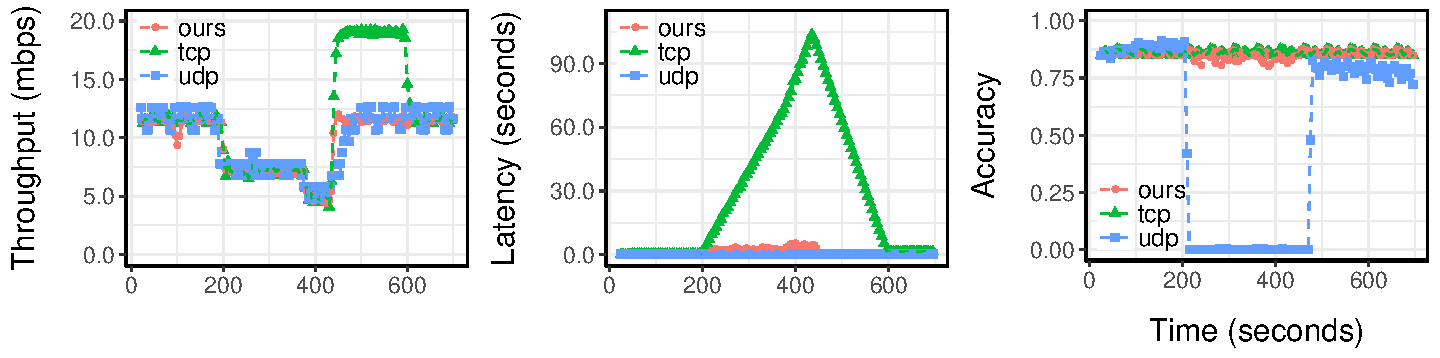
\includegraphics[width=0.95\textwidth]{figures/ped-runtime-horizontal.pdf}
  \caption{Runtime Adaptation of Pedestrian Detection}
  \label{fig:ped-runtime}
\end{figure*}

\begin{figure*}
  \centering
  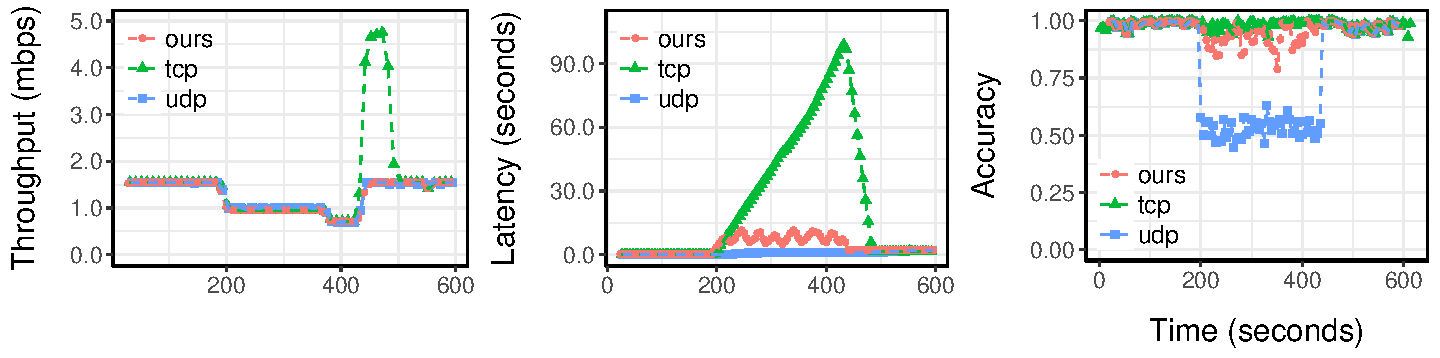
\includegraphics[width=0.95\textwidth]{figures/cdn-runtime-horizontal.pdf}
  \caption{Runtime Adaptation of Top-K}
  \label{fig:ped-runtime}
\end{figure*}

To evaluate the runtime behavior, we conduct controlled experiments using four
geo-distributed worker nodes from Amazon EC2 (t2.large instances) and an
aggregation server from our institute. For each experiment, worker nodes
transmit test data for about 10 mins. During each session, we use Linux
\texttt{tc} utility to adjust outgoing bandwidth to experiment with network
resource variation.

We compare our system with baseline systems that directly uses TCP and UDP. In
all three applications, the raw data streams are orders of magnitude
larger. While our system can adapt the rate, it could be unfair to baseline
solutions. We adjust the default degradation operation so that TCP and UDP would
work just fine when in normal cases; in this way, we make fair comparison. In
the case of UDP, shaping at the source doesn't emulate the packet loss behavior
with out-of-order delivery. We use \texttt{netem} to control packet loss rate to
match the desired shaping bandwidth.

In all three experiments, we see long delays in TCP. It increases linearly when
the traffic shaping started. When the bandwidth shaping stops, TCP quickly fills
the connection to recover. Depending on the queued size, the recovery could take
a few minutes or tens of seconds.

For UDP, the latency has been consistently small (mostly below 1 second) because
there is no queue building up. But when traffic shaping starts, the accuracy
drop is catastrophic.

Applications built with \sysname{} performs with a middle-ground behavior
between two extremes. We notice that our delay is still on the order of ten
seconds. The reason for the slow adaptation is three-folds: (1) our current
implementation only requests for bandwidth information when congestion is
detected, the delay of getting bandwidth estimation can be large in the case of
network capacity drop; (2) we perform the bandwidth in a conservative way with
smoothing to avoid sudden spikes. While more improvements are possible, the
current settings are satisfactory.

%%% Local Variables:
%%% mode: latex
%%% TeX-master: "thesis"
%%% End:

\chapter{Thesis Plan}
\label{cha:thesis-plan}

This thesis aims to make the following statement: a system-level design that
empowers adaptation in an automatic way will enable the resilient execution of
diverse streaming applications.

The current research results presented in this manuscript, i.e.\,the proposal,
demonstrate how such a design achieves a balance between delay and application
utility in the presence of network resource variation.

The complete thesis will extend the current work to a more holistic framework.
Specifically, I plan to work on the following two directions (see
\autoref{tab:plan} for the concrete timeline):

\para{Multitask resource allocation:} Many streaming applications will co-exist
and share the infrastructure. When uncoordinated, they will compete for
resources such as the network bandwidth. While the adaptation strategy may be
optimal for each application, taking them collectively, the system may not be at
an optimal state. In this direction, I will study the multitask resource
allocation and how it can adapt each streaming applications for an overall
maximal utility.

\para{Adaptation to computing resources:} In addition to network resources, the
computing resources also have a large variation across the heterogeneous
platforms. The available platforms range from embedded devices to powerful
rack-level machines. Also, the availability of the platforms is not always
guaranteed: nodes join and leave; the connectivity may be completely cut off. In
this direction, I will study how to adapt applications to different
configurations of the computing resources.

\vspace{1.5em}
\begin{table}[h]
  \normalsize
  \centering
  \begin{tabular}{r l}
    \toprule
    \textbf{Time} & \textbf{Research Topic} \\
    \midrule
    Spring 2017 & Resource allocation among multiple streaming applications \\
    Summer 2017 & Preliminary study on adaptation to computing resources \\
    Fall 2017 & Combine network and compute resources for a holistic control plane \\
    Spring 2018 &  Finish the thesis \\
    \bottomrule
  \end{tabular}
  \caption{Thesis Timeline}
  \label{tab:plan}
\end{table}

%%% Local Variables:
%%% mode: latex
%%% TeX-master: "thesis"
%%% End:


\printbibliography

\end{document}

%%% Local Variables:
%%% mode: latex
%%% TeX-master: t
%%% End:
